%%%%%%%%%%%%%%%%%%%%%
% Experiments and Results %
%%%%%%%%%%%%%%%%%%%%%

This thesis aims to analyze the relationships between different road networks and road network similarity methods. In particular,  (1) the similarities between different road networks are determined, (2) similar road networks are clustered, (3) the correlations between the different network similarity methods used to identify the similarities between the different road networks are also determined, and (4) the similar methods are clustered. Figures \ref{fig:Road Network Similarity and Ranking} and \ref{fig:Road Network Similarity Method Correlation} show a high-level overview of the process. 

\begin{figure}[h]
\centering

\includegraphics[width=0.75\textwidth,center]{picture/network_ranking.png}
\caption[Road Network Similarity and Ranking]{Road Network Similarity and Ranking}
\label{fig:Road Network Similarity and Ranking}
\end{figure}

\begin{figure}[!ht]
\centering

\includegraphics[width=0.75\textwidth,center]{picture/ranking.png}
\caption[Road Network Similarity Method Correlation]{Road Network Similarity Method Correlation}
\label{fig:Road Network Similarity Method Correlation}
\end{figure}


\section{Grid Road Network Similarity Analysis}
\label{4.1}
This section describes the experiments to identify similar road networks with Grid patterns and structure, likewise groups of methods described in Chapter 3 that have similar behavior.

The problem to find road networks with similar structures and patterns is explicitly approached using network-similarity ranking[Soundarajan]. Firstly, a reference network Gr and a collection of comparison networks H1, H2,...., Hk are given. A network-similarity method is then used to calculate the similarity between Gr and each Hi. The data (similarity scores) for each comparison are normalized for uniformity before being used to create a dendrogram. This will cancel out the effects of outliers and ensure that the results have the same units. In Table 4.1 that shows the similarity score for each comparison, the normalization is accomplished by calculating Z scores for each similarity score in each column: z = (x mean)/std. As a result, the column mean is subtracted from each value in the column and then divided by the standard deviation. As a result, all the columns have the same mean and variance. The normed values indicate how many standard deviations any individual value deviates from the column mean. The hierarchical clustering algorithm can now be used in conjunction with the Ward variance minimization algorithm by combining the linkage function to generate the dendrogram. 

The District of Columbia (USA) is chosen as the reference network for the Grid road similarity analysis, and the methods are used to compare the other networks to the reference network and generate a numerical similarity score. The networks are then clustered in hierarchical order. The goal is to see if certain road networks are similar to the reference network's Grid pattern, which generates a dendrogram with road network patterns that are similar to the reference road network pattern. The results for this analysis are presented in Figure \ref{fig:Hierarchical Clustering Dendrogram for Grid Road Networking Similarity}.

\begin{figure}[!ht]
\centering
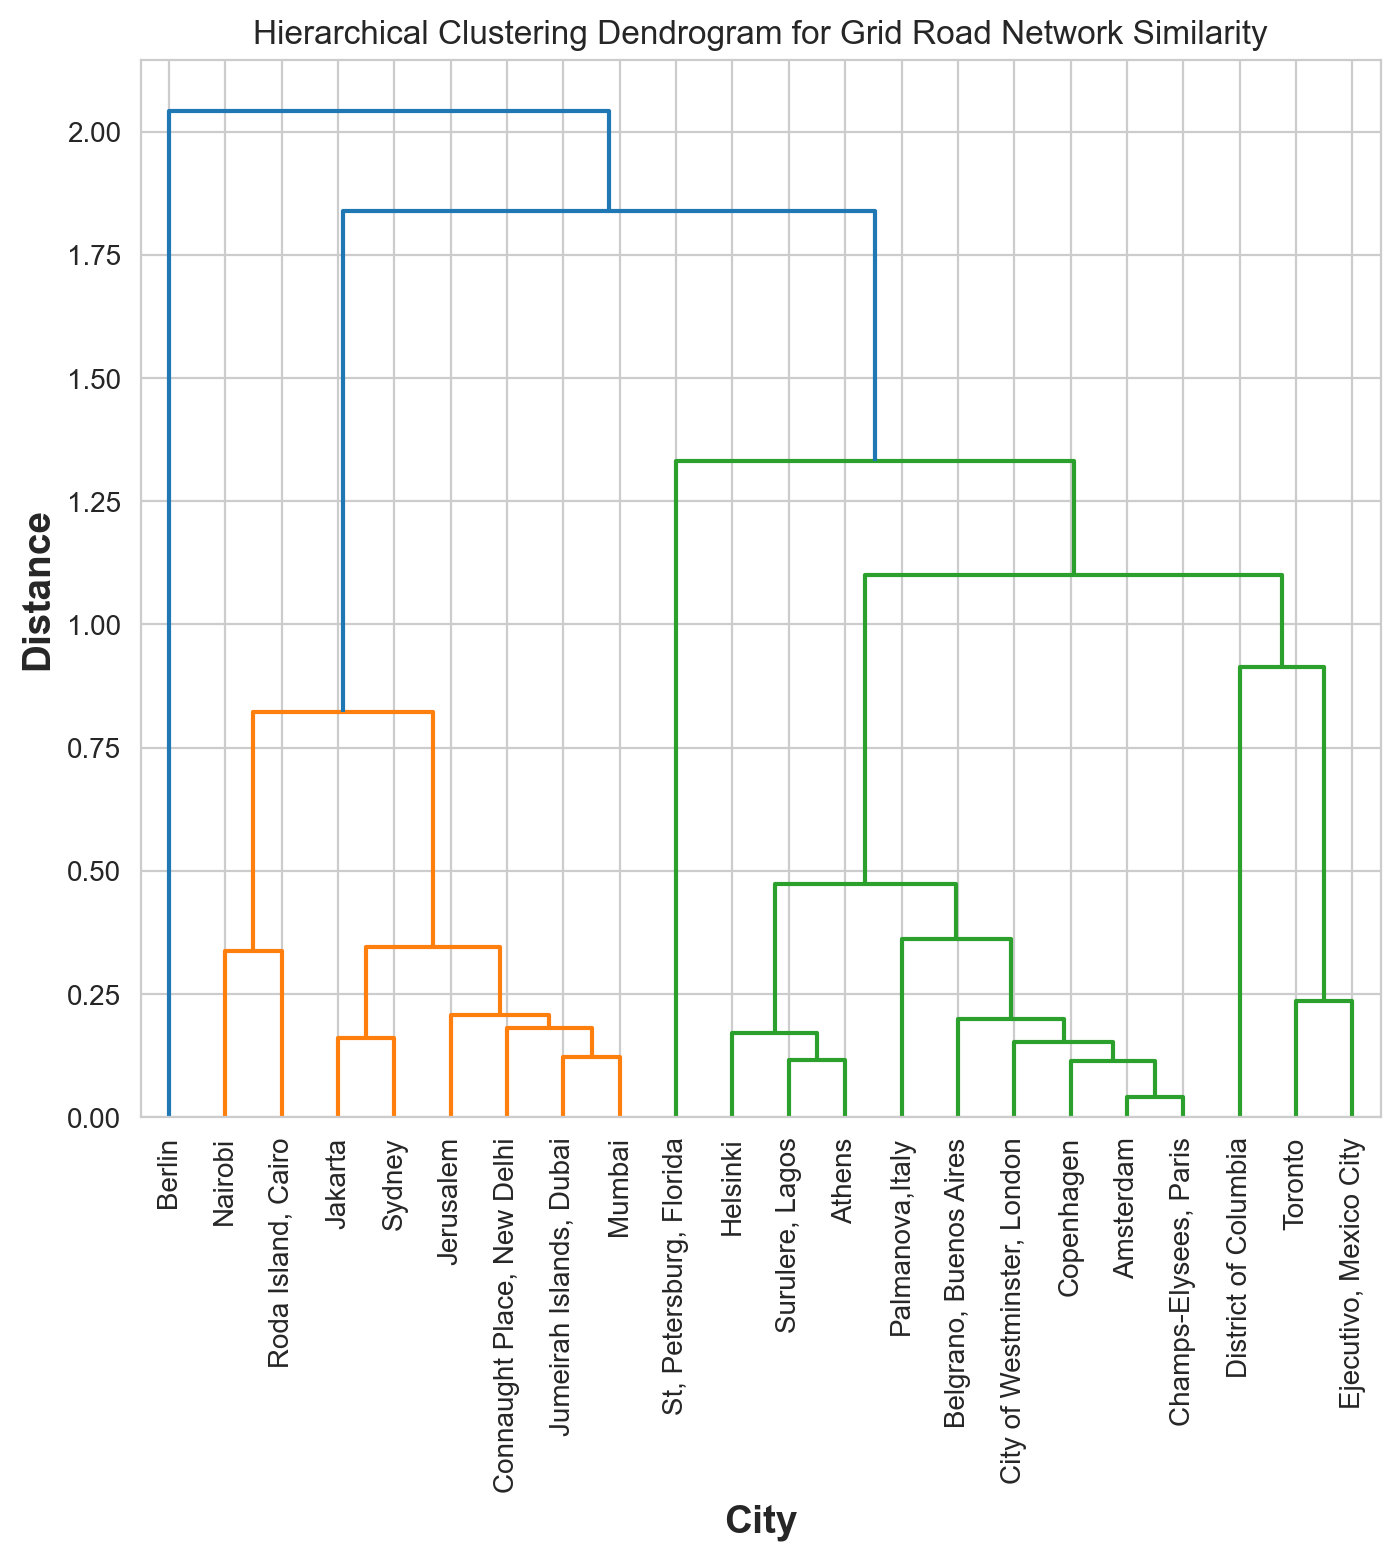
\includegraphics[width=0.75\textwidth,center]{picture/Grid/grid_dendrogram2.png}
\caption[Hierarchical Clustering Dendrogram for Grid Road Networking Similarity]{Hierarchical Clustering Dendrogram for Grid Road Networking Similarity}
\label{fig:Hierarchical Clustering Dendrogram for Grid Road Networking Similarity}
\end{figure}

Figure \ref{fig:Hierarchical Clustering Dendrogram for Grid Road Networking Similarity} presents the dendrogram obtained from the cluster analysis. The dendrogram  is interpreted using two criterias. First, a branch or cluster that includes the reference network. Second, the arrangement of the clusters which tells us the road networks that are most similar to each other, as the height of the cluster measured in distance, indicates how similar or different the road networks are from each other. The greater the distance, the greater the difference. 

For the first criteria, two major clusters (Green and Orange) can be observed from the dendrogram's structure except for the outlier; berlin road network (Blue). Looking at the green cluster, the road network for the cities Ejecutivo and Toronto lie near the reference network: District of Columbia (USA) in one adjacent cluster and are later grouped as a single cluster which indicates that this cities are the most pronounced grid-like structure similar to the reference network. 

Interpreting the dendrogram using the second criteria, the road networks for the cities Champs-Elysees, Paris and Amsterdam, Netherlands are said to be clustered first as they tend to have the cluster with the relatively shortest distance. Therefore they are the most similar than any other cluster of road networks at a higher level.

Initially, one will expect that the road networks within the green cluster should have similarities to the grid pattern of the reference network, likewise have clusters with the shortest distance, but by cross-checking with the similarity scores for each method included in the heatmap in figure \ref{fig:Heatmap showing the correlations for Grid Road Networks}, it is possible to identify the characteristics of each cluster and why certain clusters are grouped together.

\begin{figure}[!ht]
\centering
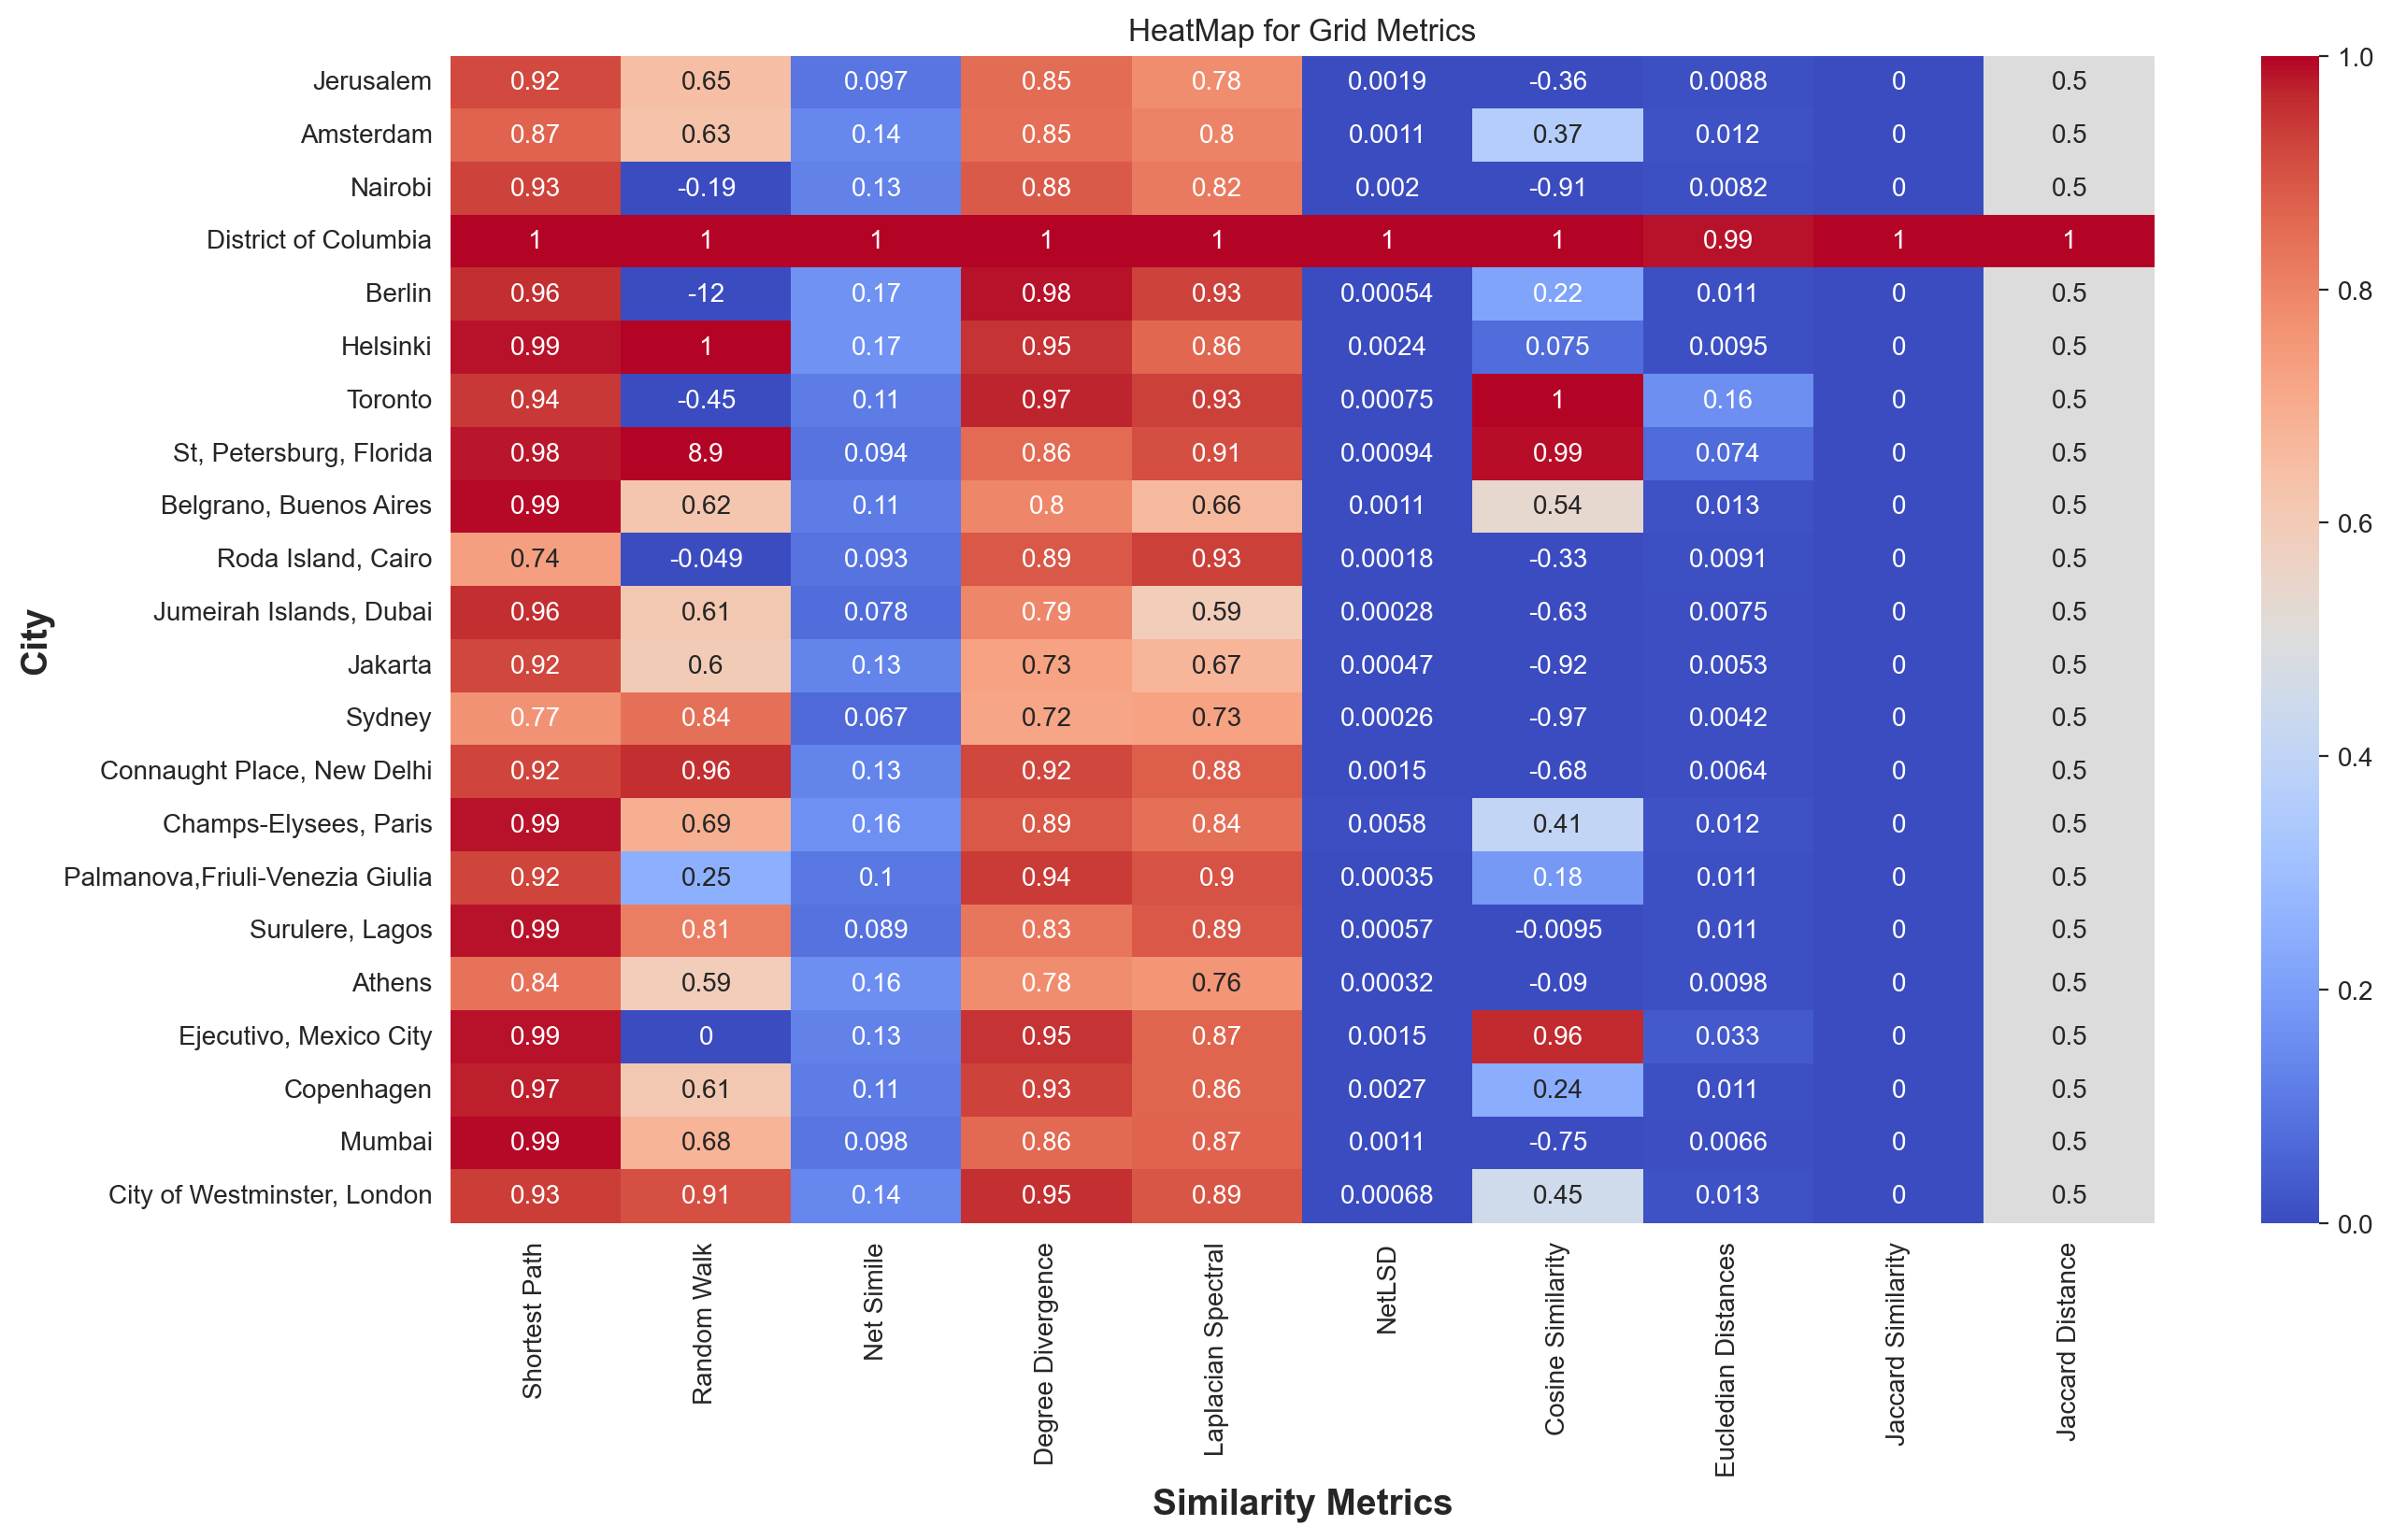
\includegraphics[width=0.85\textwidth,center]{picture/Grid/gridheatmap.png}
\caption[Heatmap showing the correlations for Grid Road Networks]{Heatmap showing the correlations between the road networks when the road network: District of Columbia was used as the reference network.}
\label{fig:Heatmap showing the correlations for Grid Road Networks}
\end{figure}


A major challenge observed while using dendrograms to visualize the hierarchical clustering is that; dendrograms only tell us a little bit about the similarities of road networks based on the clusters generated. The dendrogram clearly depicts a different picture, with some road networks grouped differently (see how the distribution of the road networks is mixed). For example, St. Petersburg, Florida, which is considered to be among the most similar to the reference network based on the similarity scores in figure \ref{fig:Heatmap showing the correlations for Grid Road Networks}, is later combined with the clusters of Ejecutivo, Toronto, and the District of Columbia (USA). As the dendrogram results are not intuitive, it is not suitable for interpreting the similarity results. Further analysis or another alternative to visualize the results of the similar scores is recommended to possibly identify the groups of clusters with road networks that behave similarly.

In addition, dendrograms only tell us a bit in terms similarities of road networks based on the clusers generated. The dendrogram clearly shows a different picture, where some of the road networks are grouped differently (see how the distribution of the road networks is mixed). For example, St, Petersburg, Florida which from the similarity scores in figure \ref{fig:Heatmap showing the correlations for Grid Road Networks} considered to be amongst the most similar to the reference network is later put together with cluster of Ejecutivo, Toronto and the District of Columbia (USA). Further analysis is recommended or another alternative to visualize the results of the similar scores is recommended as the dendrogram results are not intuitive, thus making it not suitable for interpreting the similarity results.

To find methods that behave similarly, the pairwise Kendall-Tau distance between each pair of methods is calculated first, followed by a complete-linkage hierarchical clustering because it produces a dendrogram with many small clusters, which provides insight into which groups of methods are closely correlated.

\begin{figure}[!ht]
\centering
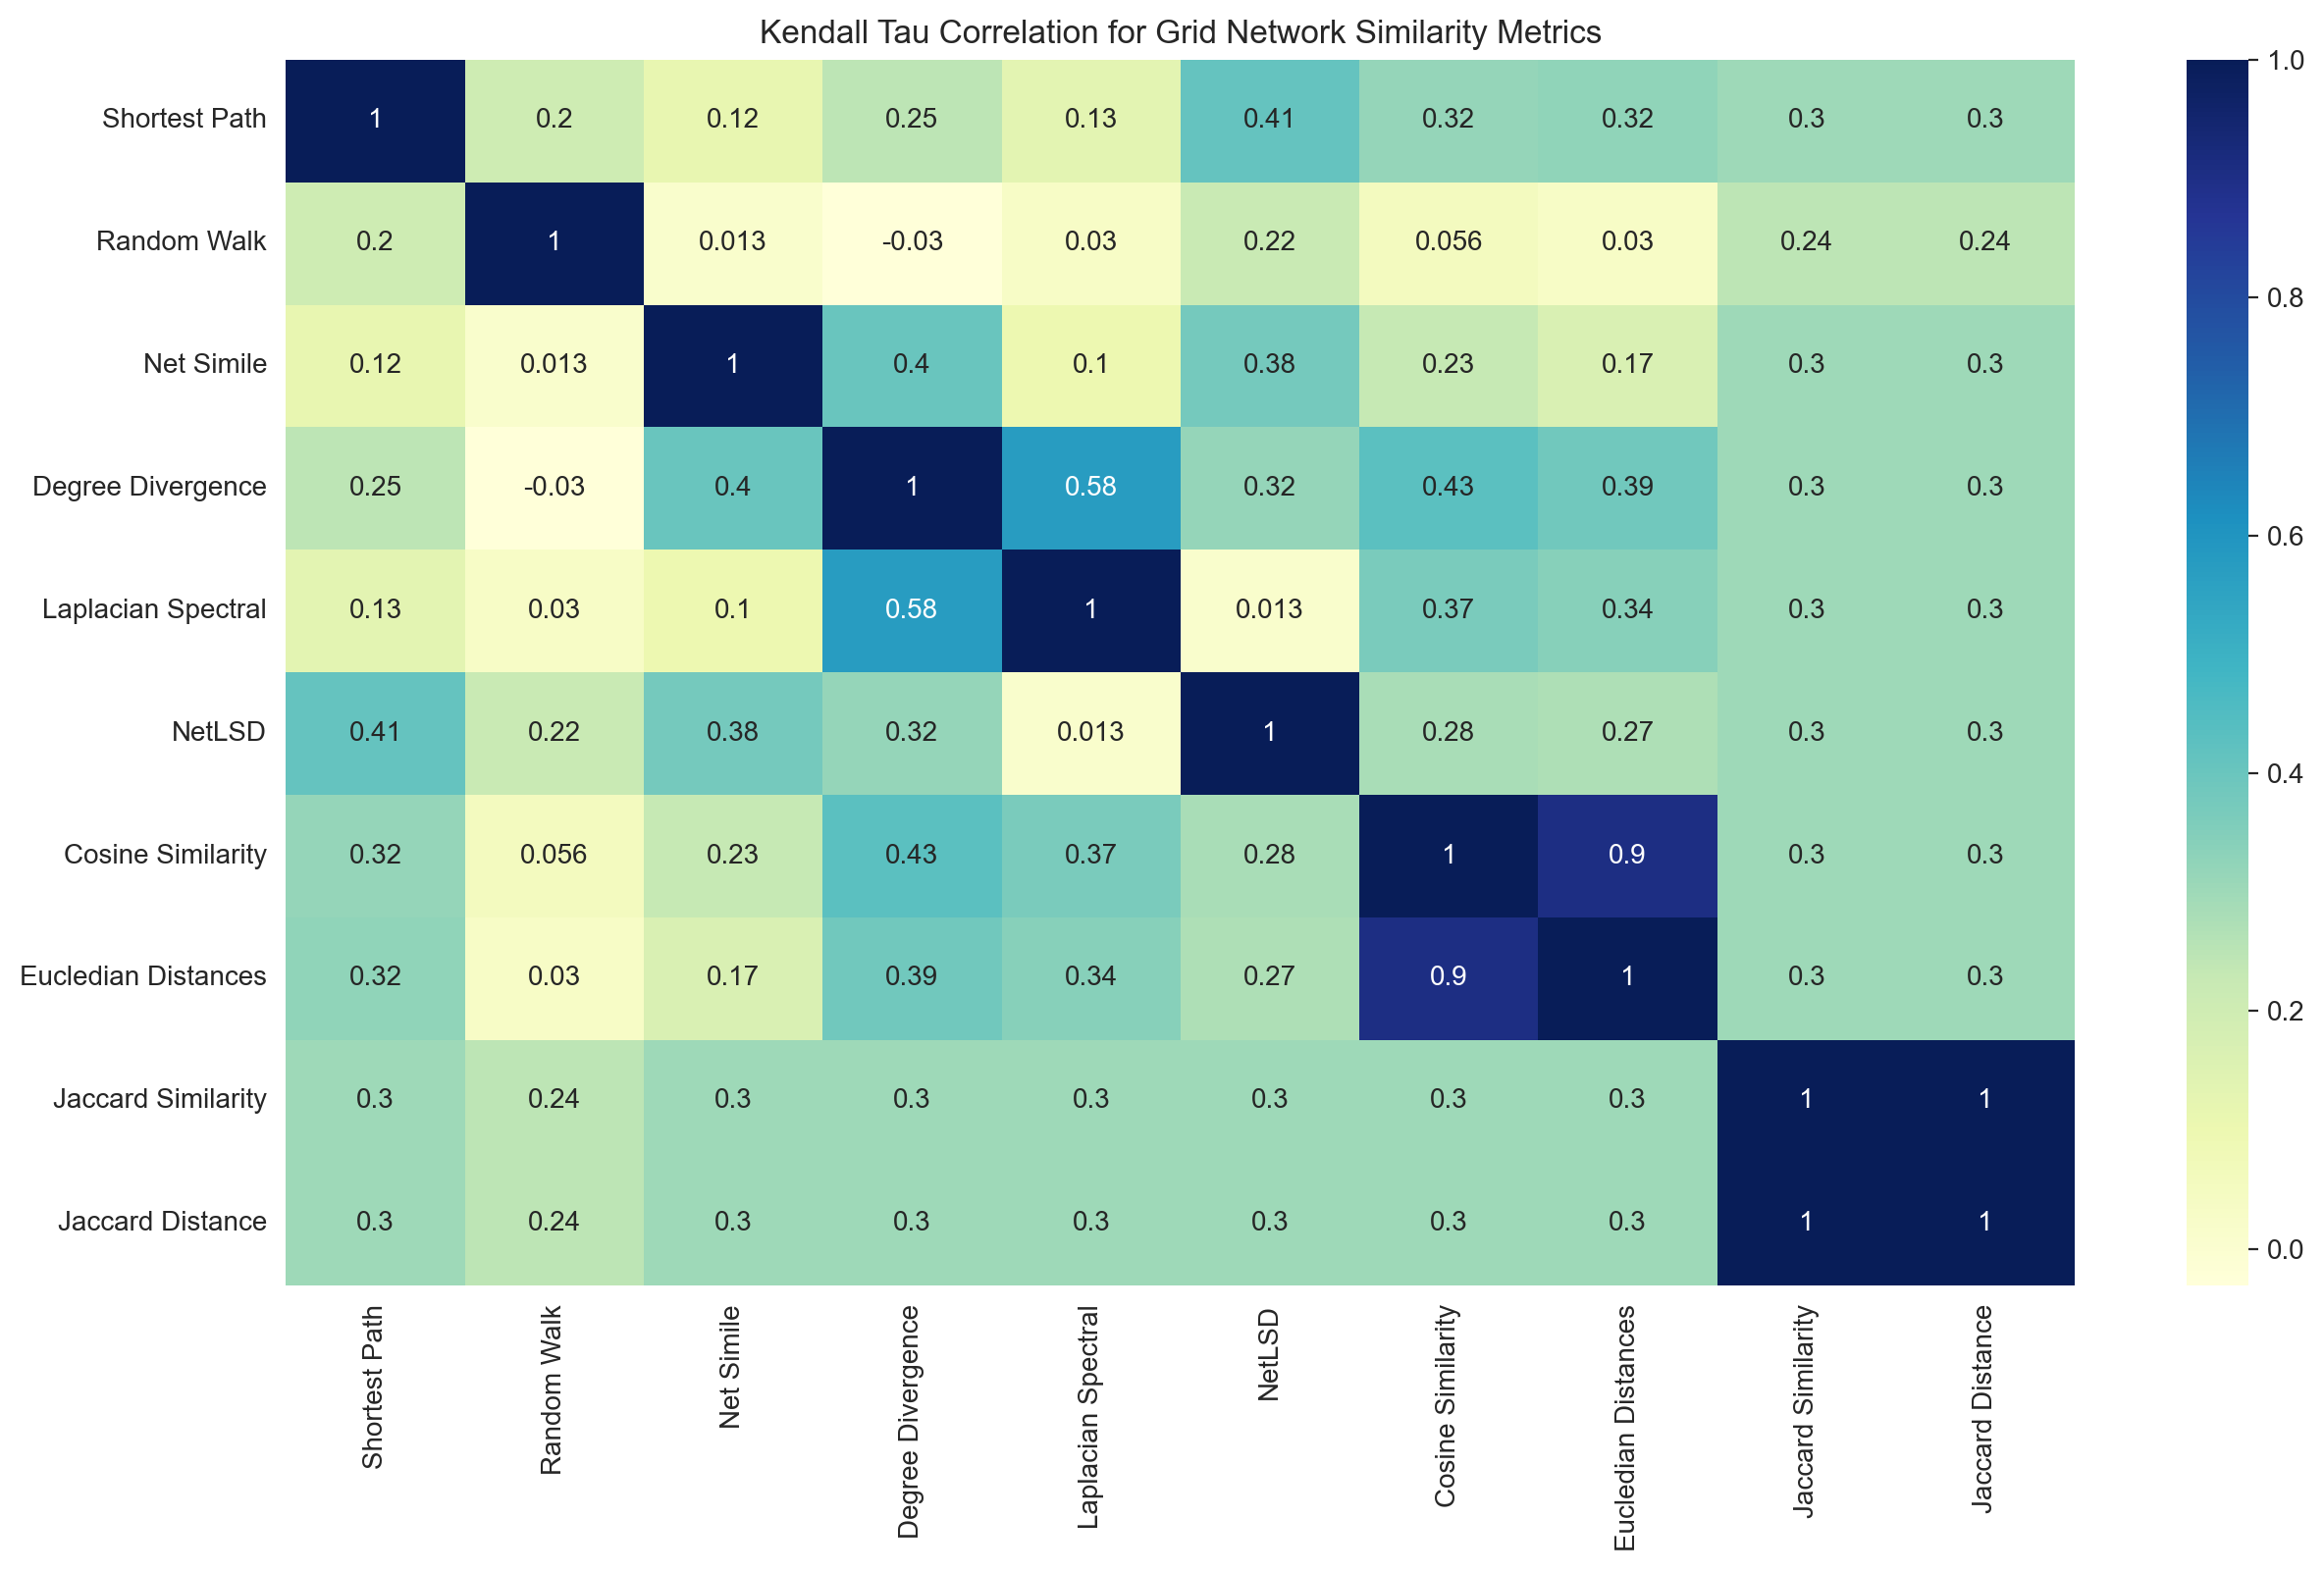
\includegraphics[width=0.85\textwidth,center]{picture/Grid/grid2.png}
\caption[Heatmap showing Kendall-Tau correlations between the road network similarity methods for Grid Road Networks]{Heatmap showing Kendall-Tau correlations between the road network similarity methods when the road network: District of Columbia was used as the reference network.}
\label{fig:network ranking}
\end{figure}

Each square illustrates the relationship between the variables on each axis. Correlation values range from 0 to 1. Values close to zero indicate that there is no linear relationship between the two variables. The closer the correlation is to one, the more positively correlated they are; that is, as one increases, so does the other, and the closer to one, the stronger the relationship. A correlation closer to 0 is similar, but instead of both variables increasing, one variable decreases as the other increases. The diagonals are all 1/dark blue because those squares are perfectly correlating each variable to itself. For the rest, the higher the correlation between the two variables, the larger the number and the darker the color. Because the same two variables are paired together in those squares, the plot is also symmetrical about the diagonal.

The Kendall-Tau distances between the scores produced by the different methods when comparing road networks similar to the reference network with a Grid pattern are shown in figure \ref{fig:network ranking}. When both the Jaccard Distance and the Jaccard Similarity are used, the results show a positive correlation of 1. This is to be expected given that the Jaccard Distance is thought to be complementary to the Jaccard Similarity, which is obtained by subtracting the Jaccard coefficient from 1. With a correlation of 0.9, the methods cosine similarity and euclidean distance also behave similarly. As shown in table \ref{tab:Road Network Similarity Methods}, both methods are vector-based and operate at the micro level. This implies that when calculating vector-based similarity on road networks at the Micro-level, either of the two methods could be used. However, there is a pronounced weaker correlation between the other methods because the level of the network they operate on and the type of comparison they use are different.

Next, the methods are clustered using complete linkage hierarchical clustering on the pairwise Kendall Tau distances, as one of the goals of using this approach is to determine whether certain network similarity methods are associated with each other. The dendrogram results are presented in the appendix section.


\section{Radial Road Network Similarity Analysis}

The Connaught Place, New Delhi is chosen as the reference network for the Radial road similarity analysis, and the methods are used to compare the other networks to the reference network and generate a numerical similarity score. The networks are then clustered in hierarchical order. The results for this analysis are presented in Figure \ref{fig:Hierarchical Clustering Dendrogram for Radial Road Networking Similarity}.

\begin{figure}[!ht]
\centering
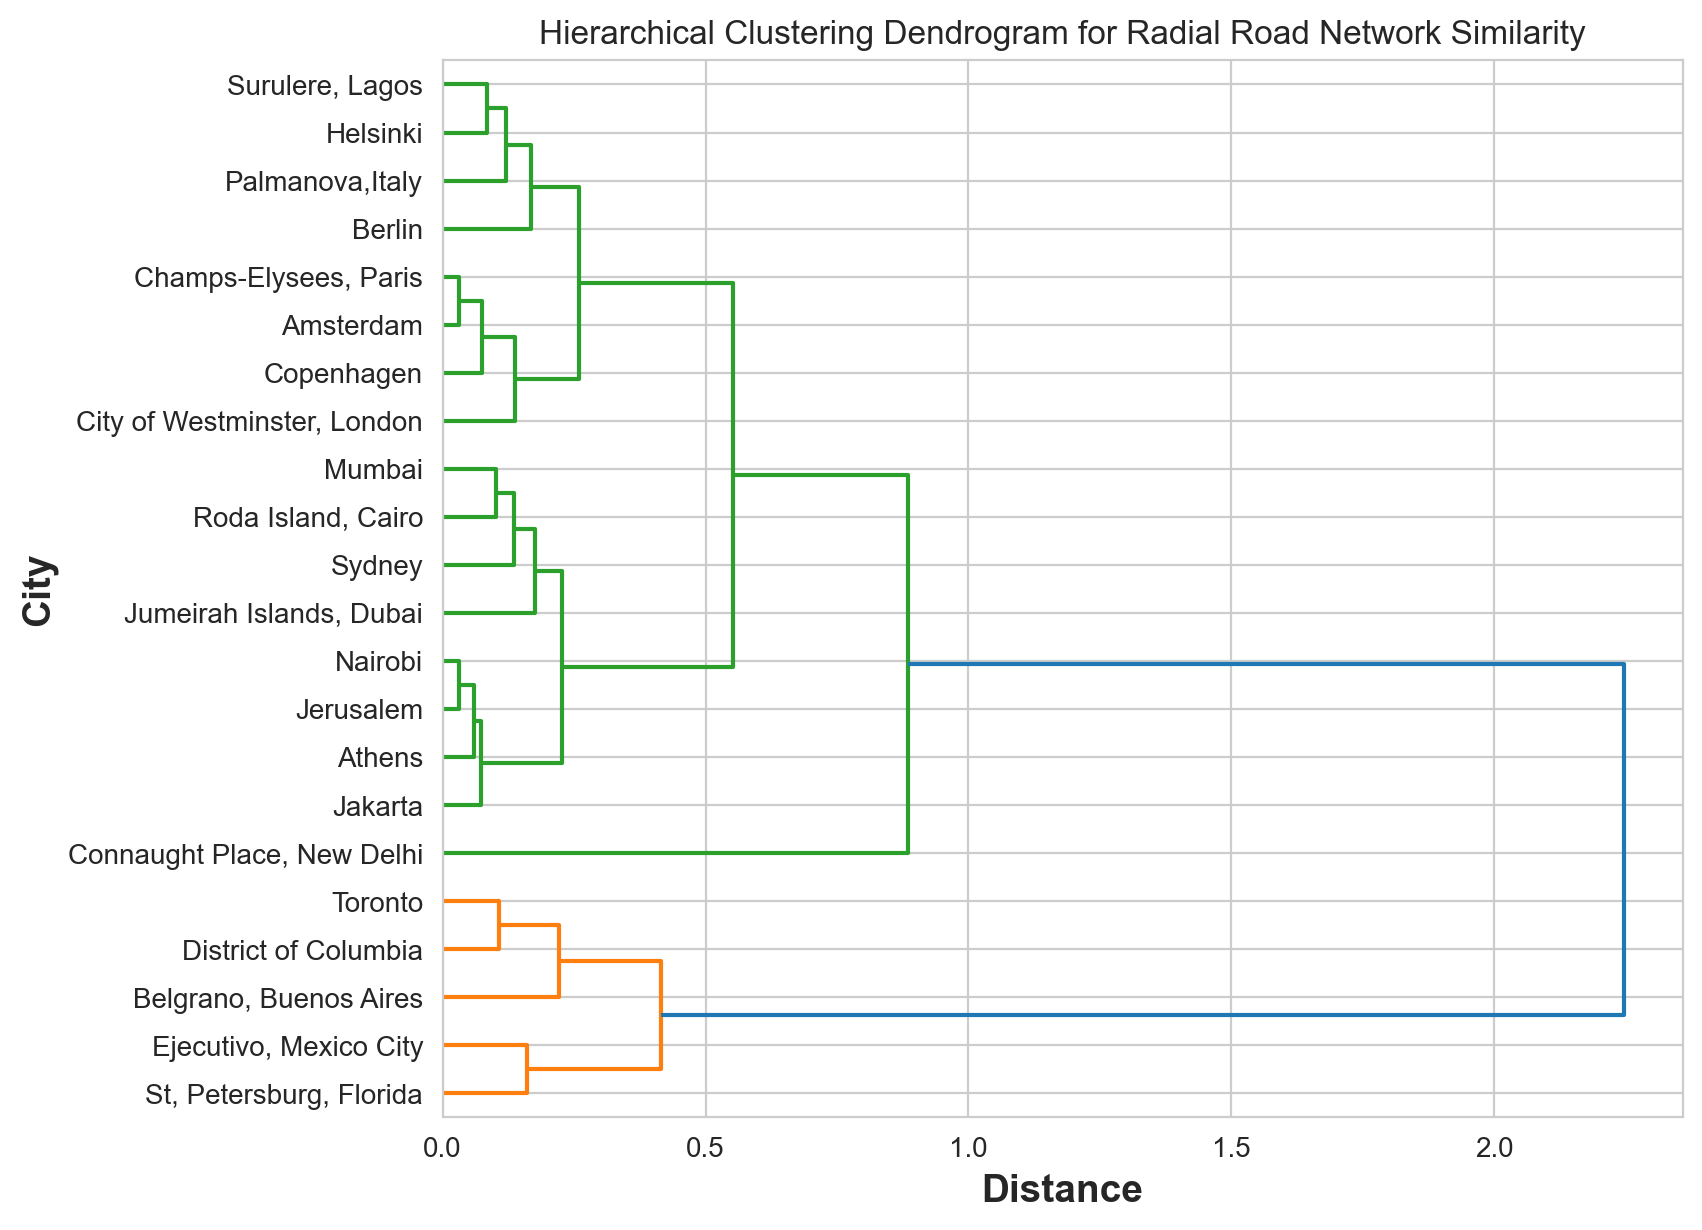
\includegraphics[width=0.75\textwidth,center]{picture/Radial/radial_dendrogram2.png}
\caption[Hierarchical Clustering Dendrogram for Radial Road Networking Similarity]{Hierarchical Clustering Dendrogram for Radial Road Networking Similarity}
\label{fig:Hierarchical Clustering Dendrogram for Radial Road Networking Similarity}
\end{figure}

Figure \ref{fig:Hierarchical Clustering Dendrogram for Radial Road Networking Similarity} presents the dendrogram obtained from the cluster analysis. The dendrogram is interpreted using the two criterias as described in Section 4.1.

For the first criteria, two major clusters (Green and Orange) can be observed from the dendrogram's structure. Looking at the green cluster, there are no road networks that lie near the reference network. However, all Road network patterns identified using the Grid network analysis with the most pronounced grid-like structure are clustered together (Orange Cluster). 

Interpreting the dendrogram using the second criteria, the road networks for the cities Champs-Elysees, Paris and Amsterdam, Netherlands are said to be clustered first as they tend to have the cluster with the relatively shortest distance followed by the cities Nairobi and Jerusalem as they are the most similar than any other cluster of road networks.

In comparison to the Grid Network Analysis, most of the road networks with similar patterns to the reference network with a radial like structure lie within the same cluster(green) with shorter distances while the road networks with not so similar patterns are clustered separately (orange cluster). This is expected because by cross-checking with the similarity scores for each method included in the heatmap in figure \ref{fig:Heatmap showing the correlations for Radial Road Networks}, and the structure of the graphs in figure \ref{fig:roadnetworkgraphs}it is possible to identify the characteristics of each cluster and why certain clusters are grouped together.

\begin{figure}[!ht]
\centering
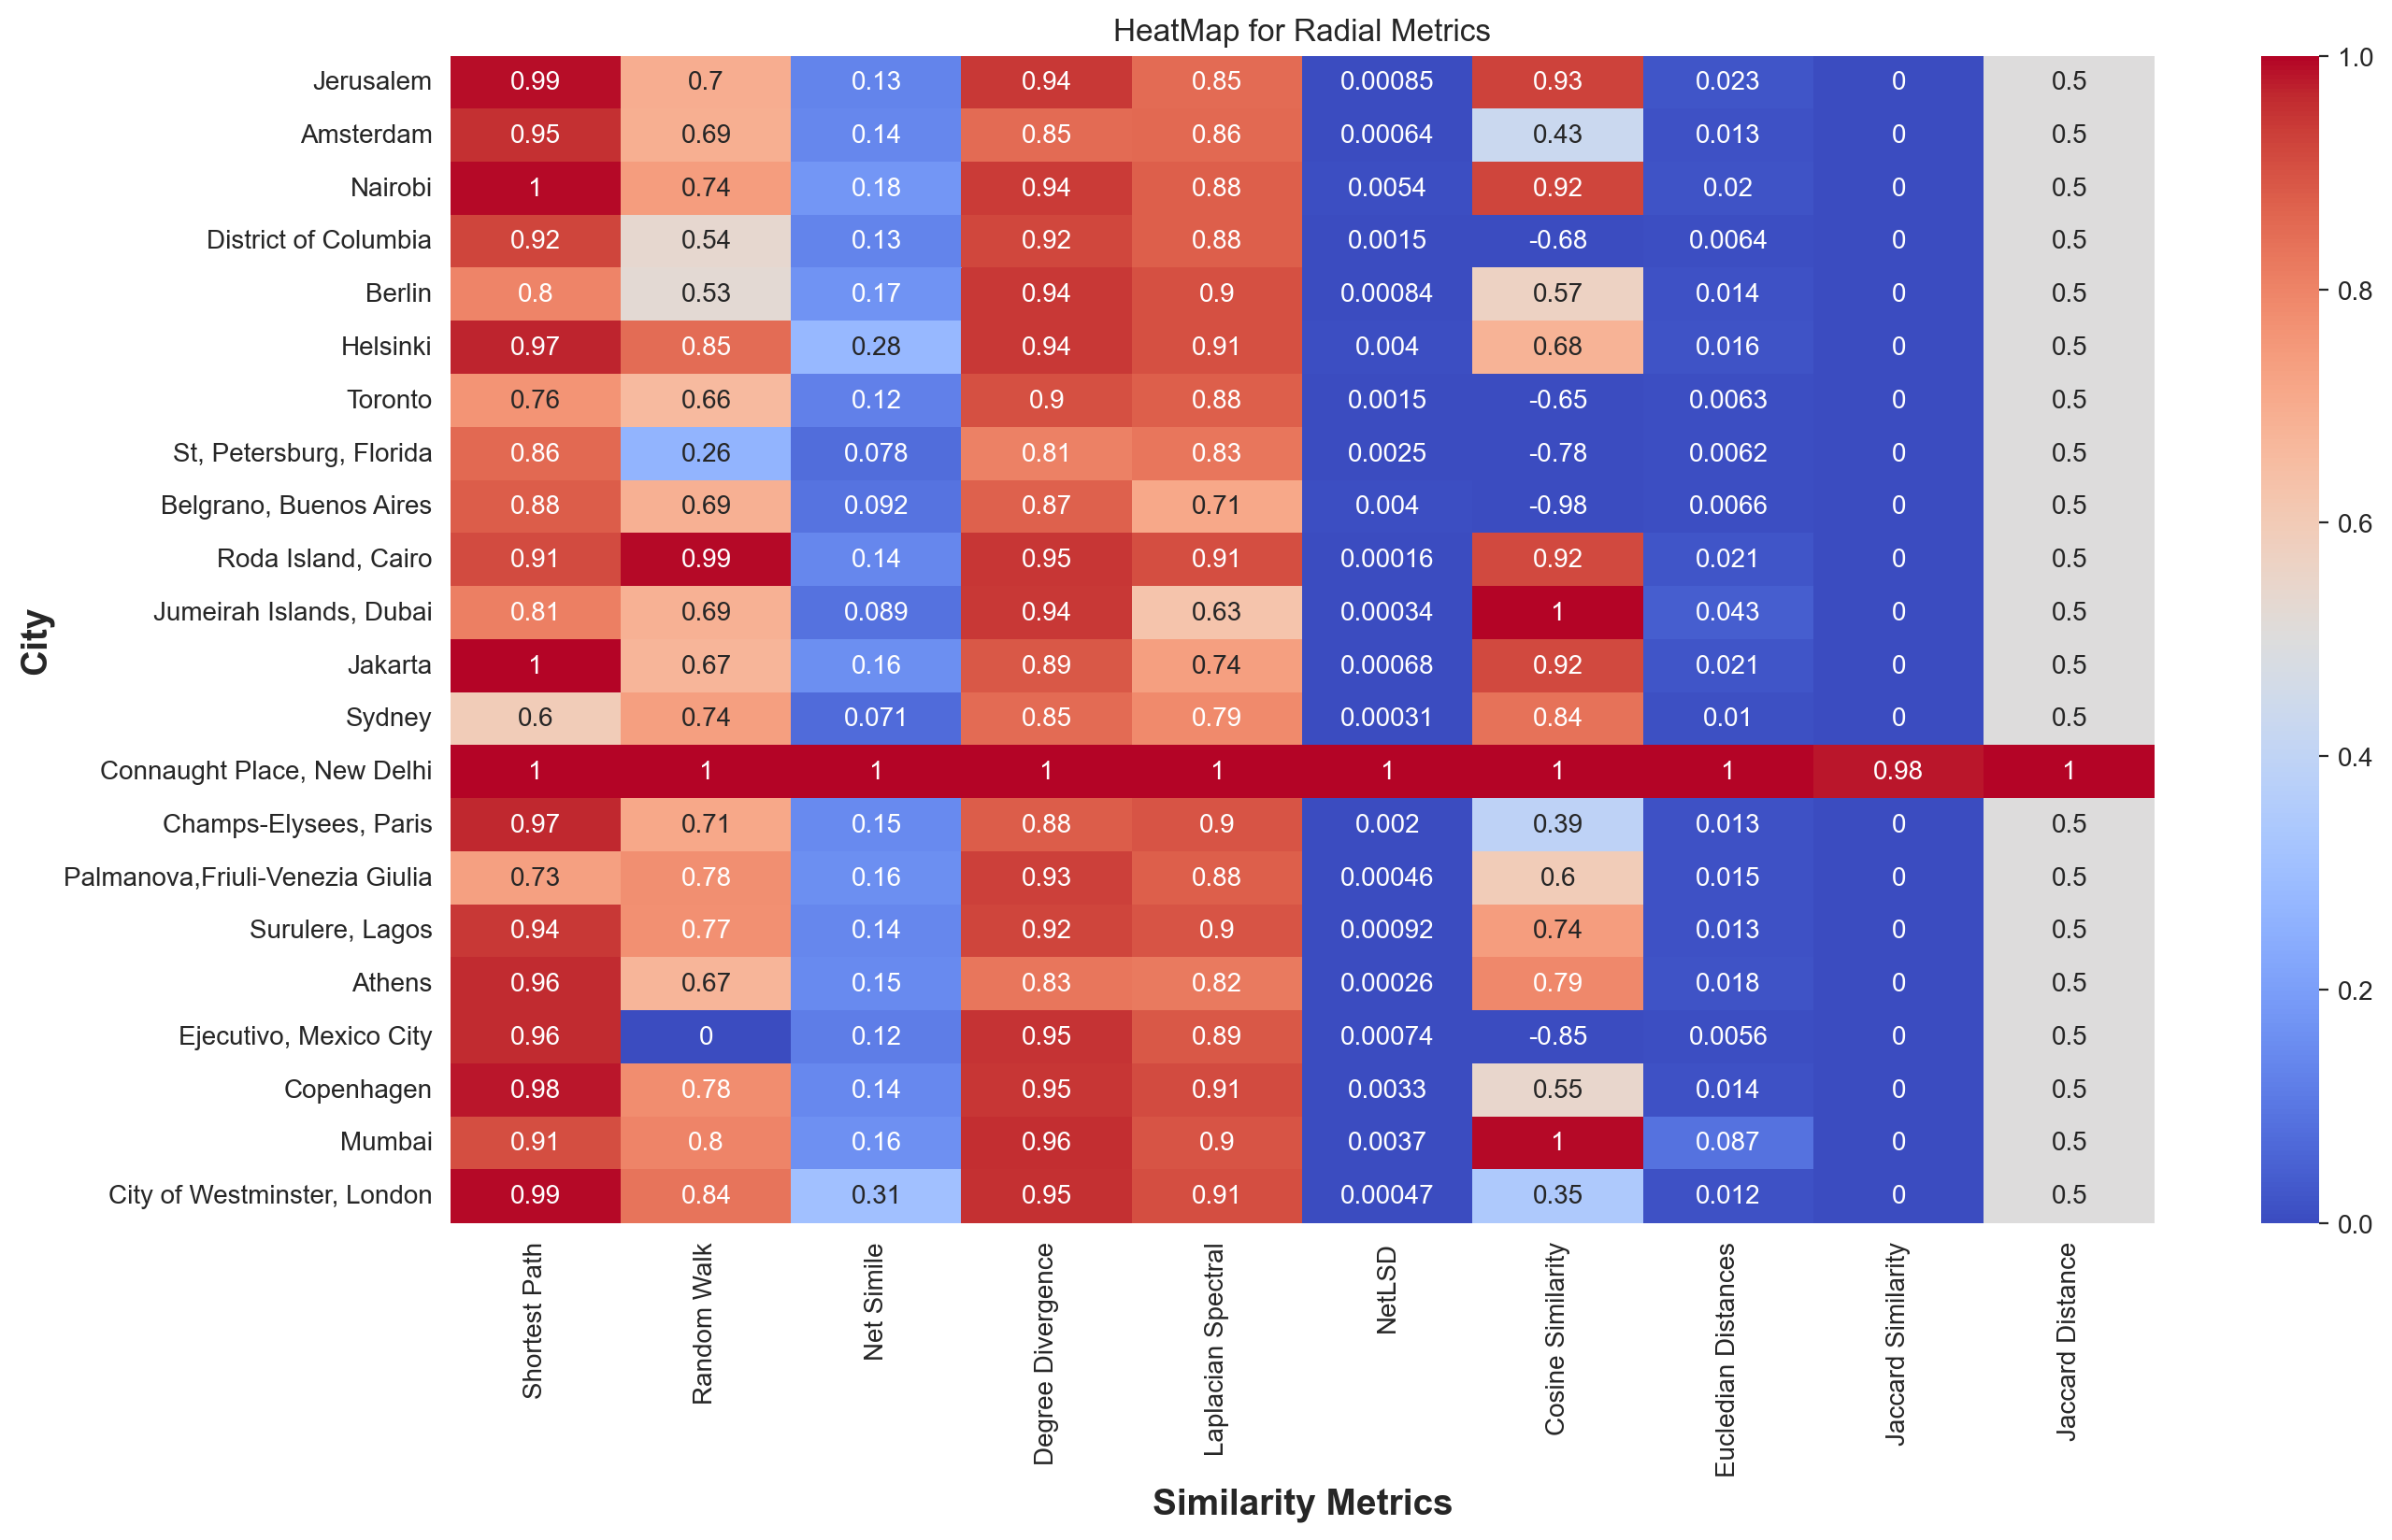
\includegraphics[width=0.85\textwidth,center]{picture/Radial/radialheatmap.png}
\caption[Heatmap showing the correlations for Radial Road Networks]{Heatmap showing the correlations between the road networks when the road network: District of Columbia was used as the reference network.}
\label{fig:Heatmap showing the correlations for Radial Road Networks}
\end{figure}


As mentioned previously, further analysis is recommended or another alternative to visualize the results of the similar scores is recommended as the dendrogram results are not intuitive, thus making it not suitable for interpreting the similarity results.

To find methods that behave similarly, the pairwise Kendall-Tau distance between each pair of methods is calculated first, followed by a complete-linkage hierarchical clustering because it produces a dendrogram with many small clusters, which provides insight into which groups of methods are closely correlated.

\begin{figure}[!ht]
\centering
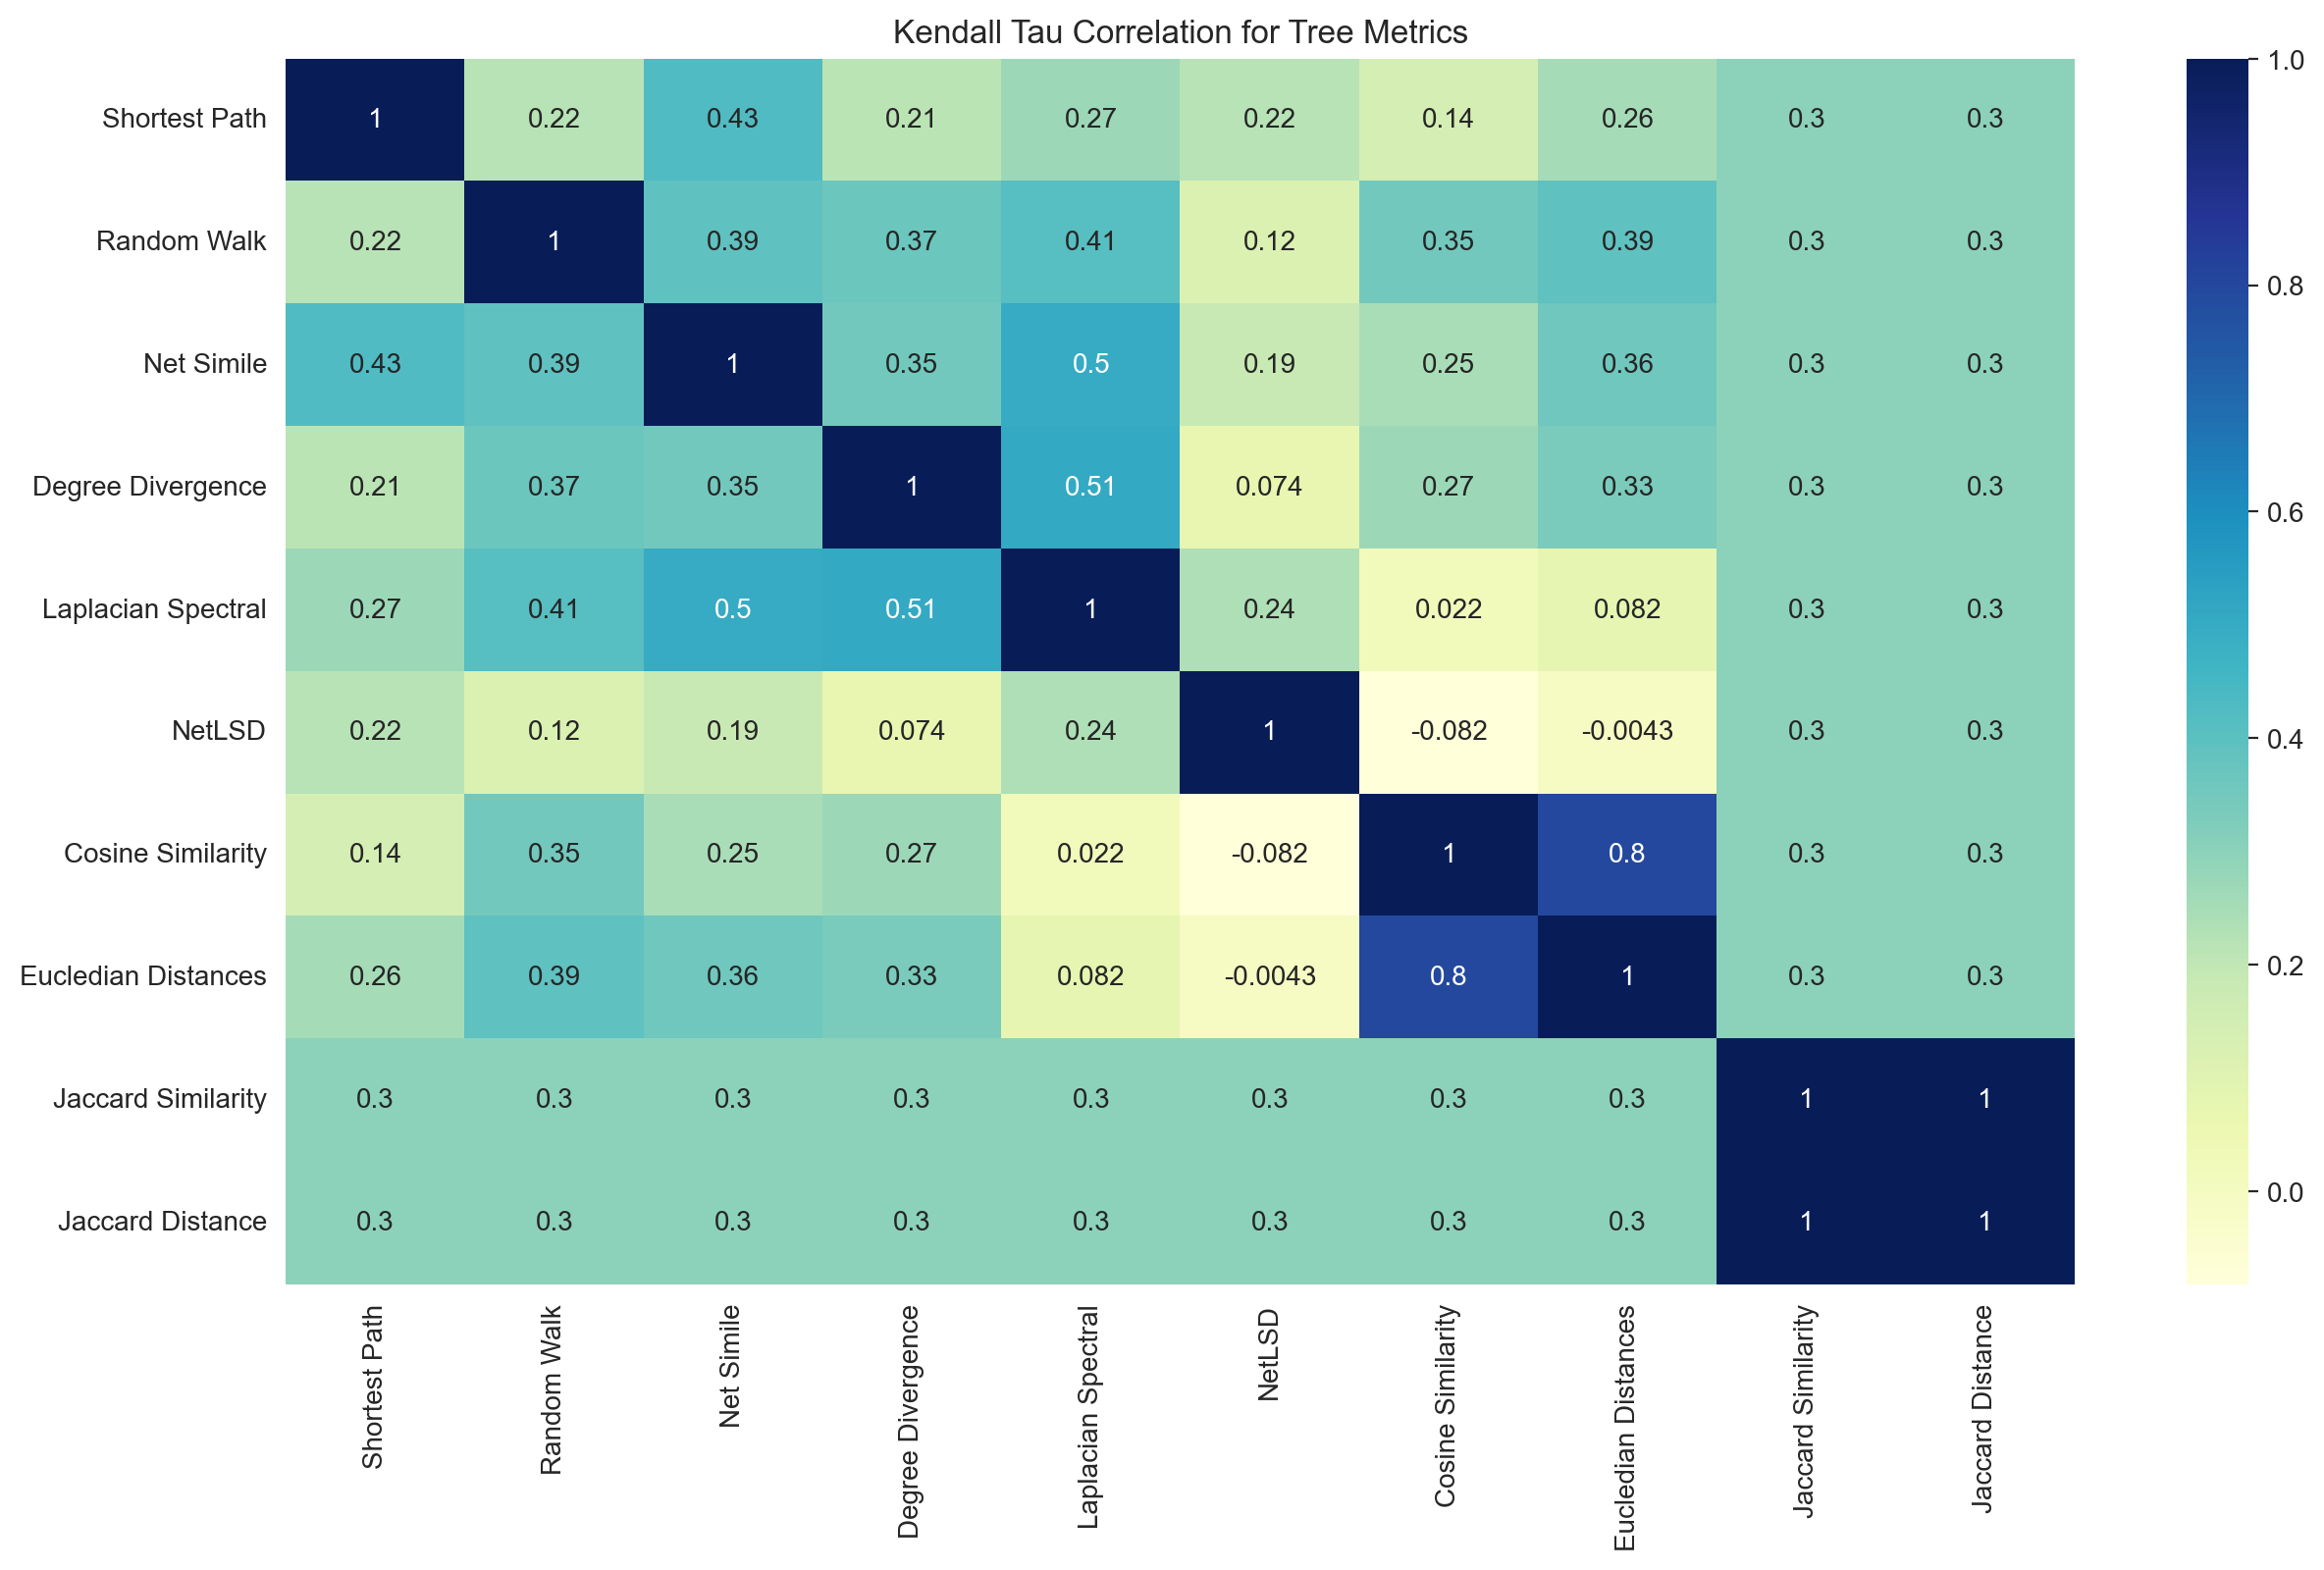
\includegraphics[width=0.85\textwidth,center]{picture/Radial/radial2.png}
\caption[Heatmap showing Kendall-Tau correlations between the road network similarity methods for Radial Road Networks]{Heatmap showing Kendall-Tau correlations between the road network similarity methods when the road network: District of Columbia was used as the reference network.}
\label{fig:network ranking radial}
\end{figure}

The Kendall-Tau distances between the scores generated by the different methods when comparing road networks similar to the reference network with a Radial like structure are shown in figure \ref{fig:network ranking radial}. When both the Jaccard Distance and the Jaccard Similarity are used, the results show a positive correlation of 1. This is to be expected given that the Jaccard Distance is thought to be complementary to the Jaccard Similarity, which is obtained by subtracting the Jaccard coefficient from 1. With a correlation of 0.8, the methods cosine similarity and euclidean distance also behave similarly. As shown in table \ref{tab:Road Network Similarity Methods}, both methods are vector-based and operate at the micro level. This implies that when calculating vector-based similarity on road networks at the Micro-level, either of the two methods could be used. However, there is a pronounced weaker correlation between the other methods because the level of the network they operate on and the type of comparison they use are different.

Next, the methods are clustered using complete linkage hierarchical clustering on the pairwise Kendall Tau distances, as one of the goals of using this approach is to determine whether certain network similarity methods are associated with each other. The dendrogram results are presented in the appendix section.


\section{Tree Road Network Similarity Analysis}

The City of Westminster, London is chosen as the reference network for the Tree road similarity analysis, and the methods are used to compare the other networks to the reference network and generate a numerical similarity score. The networks are then clustered in hierarchical order. The results for this analysis are presented in Figure \ref{fig:Hierarchical Clustering Dendrogram for Tree Road Networking Similarity}.

\begin{figure}[!ht]
\centering
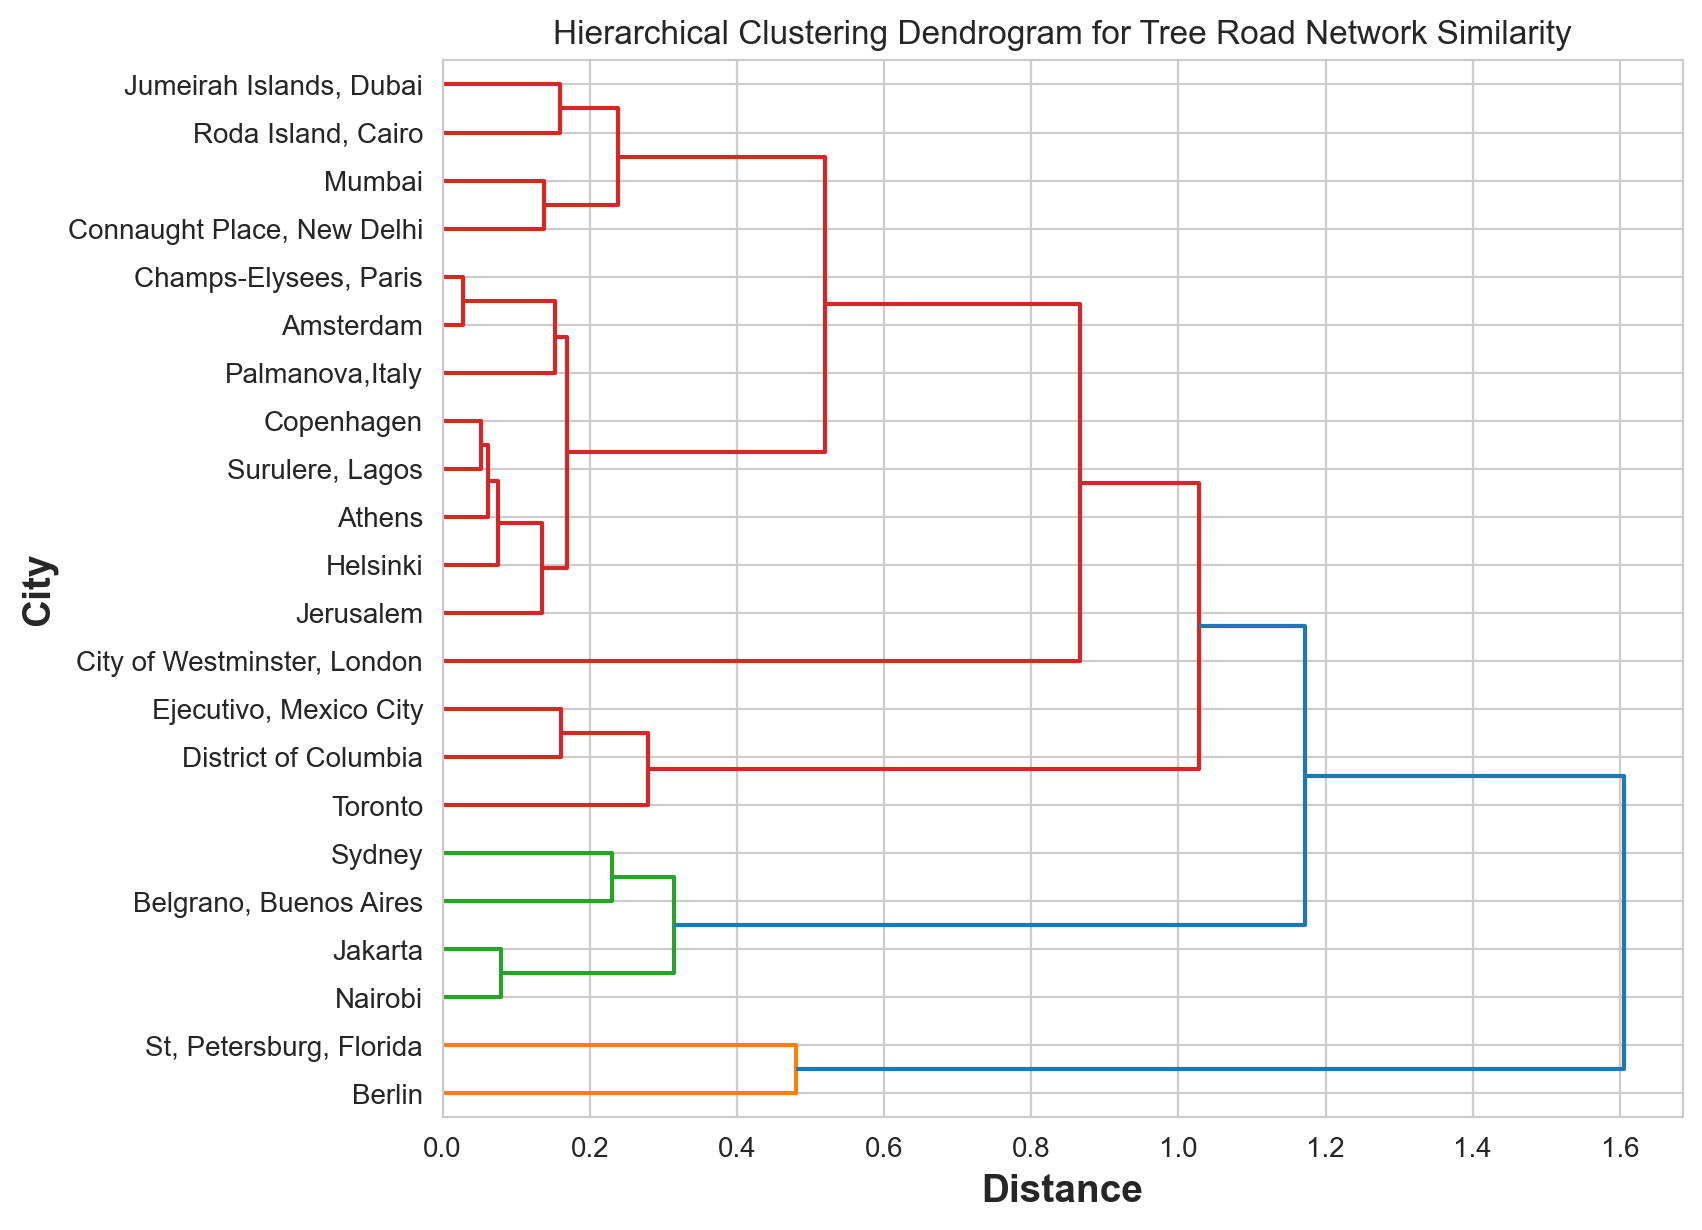
\includegraphics[width=0.75\textwidth,center]{picture/Tree/tree_dendrogram2.png}
\caption[Hierarchical Clustering Dendrogram for Tree Road Networking Similarity]{Hierarchical Clustering Dendrogram for Tree Road Networking Similarity}
\label{fig:Hierarchical Clustering Dendrogram for Tree Road Networking Similarity}
\end{figure}

Figure \ref{fig:Hierarchical Clustering Dendrogram for Tree Road Networking Similarity} presents the dendrogram obtained from the cluster analysis. The dendrogram is interpreted using the two criterias as described in Section 4.1.

The structure of the dendrogram reveals three major clusters (Red, Green, and Orange) for the first criteria. However, using the first criteria to interpret the generated clusters fails because the dendrogram results are not intuitive because some clusters contained a mix of road networks with varying structures. Berlin, for example, is in the same cluster as St. Petersburg, Florida. And, based on the heatmap similarity scores in figure \ref{fig:Heatmap showing the correlations for Tree Road Networks}, they are not expected to be in the same cluster, as is evident for other clusters as well.

Interpreting the dendrogram using the second criteria, the road networks for the cities Champs-Elysees, Paris and Amsterdam, Netherlands are said to be clustered first similar to figure \ref{fig:Hierarchical Clustering Dendrogram for Grid Road Networking Similarity} and \ref{fig:Hierarchical Clustering Dendrogram for Radial Road Networking Similarity} as they tend to have the cluster with the relatively shortest distance followed by the cities Copenhagen and Surulere, Lagos as they are the most similar than any other cluster of road networks.

In comparison to the Grid and Radial Network Analysis, the road network: Mumbai, which is identified as the other only tree road network pattern in table \ref{tab:Selected Cities}, is located within the same cluster (red), but a greater distance from the reference road network. This is to be expected because it is possible to identify the characteristics of the respective cluster and why they are not grouped together by cross-checking with the similarity scores for each method included in the heatmap in figure \ref{fig:Heatmap showing the correlations for Tree Road Networks}.


\begin{figure}[!ht]
\centering
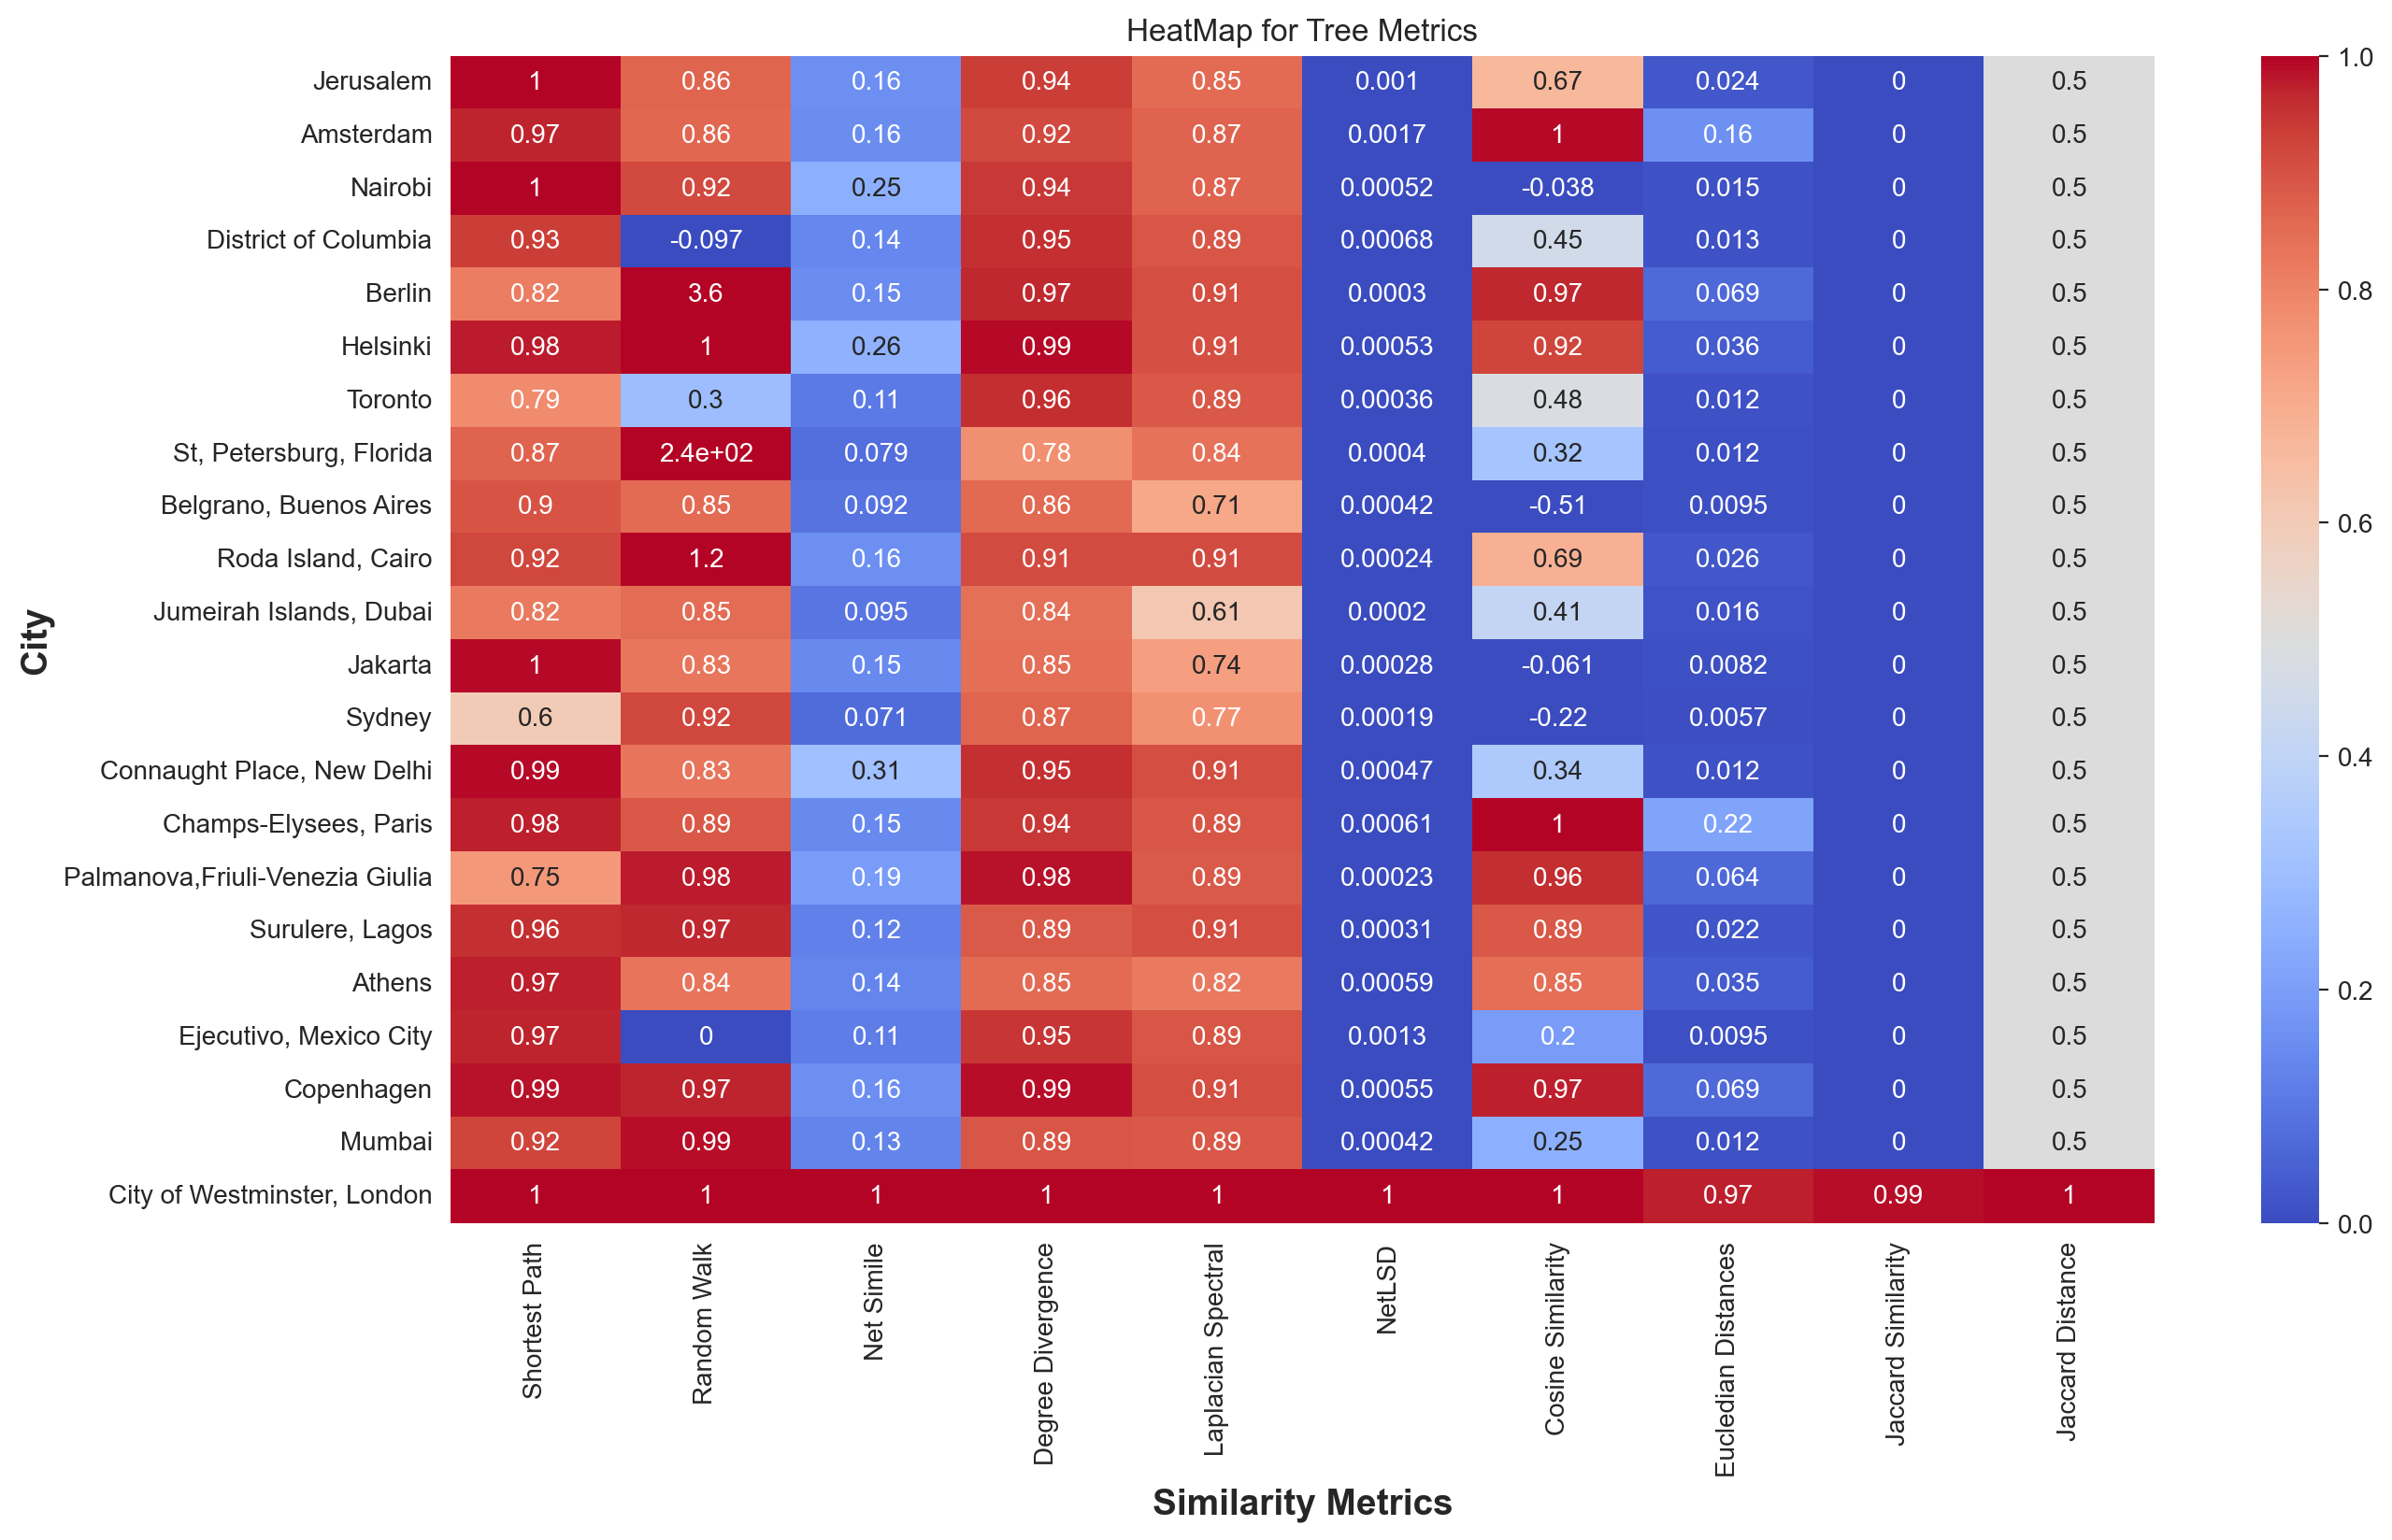
\includegraphics[width=0.85\textwidth,center]{picture/Tree/treeheatmap.png}
\caption[Heatmap showing the correlations for Tree Road Networks]{Heatmap showing the correlations between the road networks when the road network: City of Westminster, London was used as the reference network.}
\label{fig:Heatmap showing the correlations for Tree Road Networks}
\end{figure}

To find methods that behave similarly, the pairwise Kendall-Tau distance between each pair of methods is calculated first, followed by a complete-linkage hierarchical clustering because it produces a dendrogram with many small clusters, which provides insight into which groups of methods are closely correlated.

\begin{figure}[!ht]
\centering
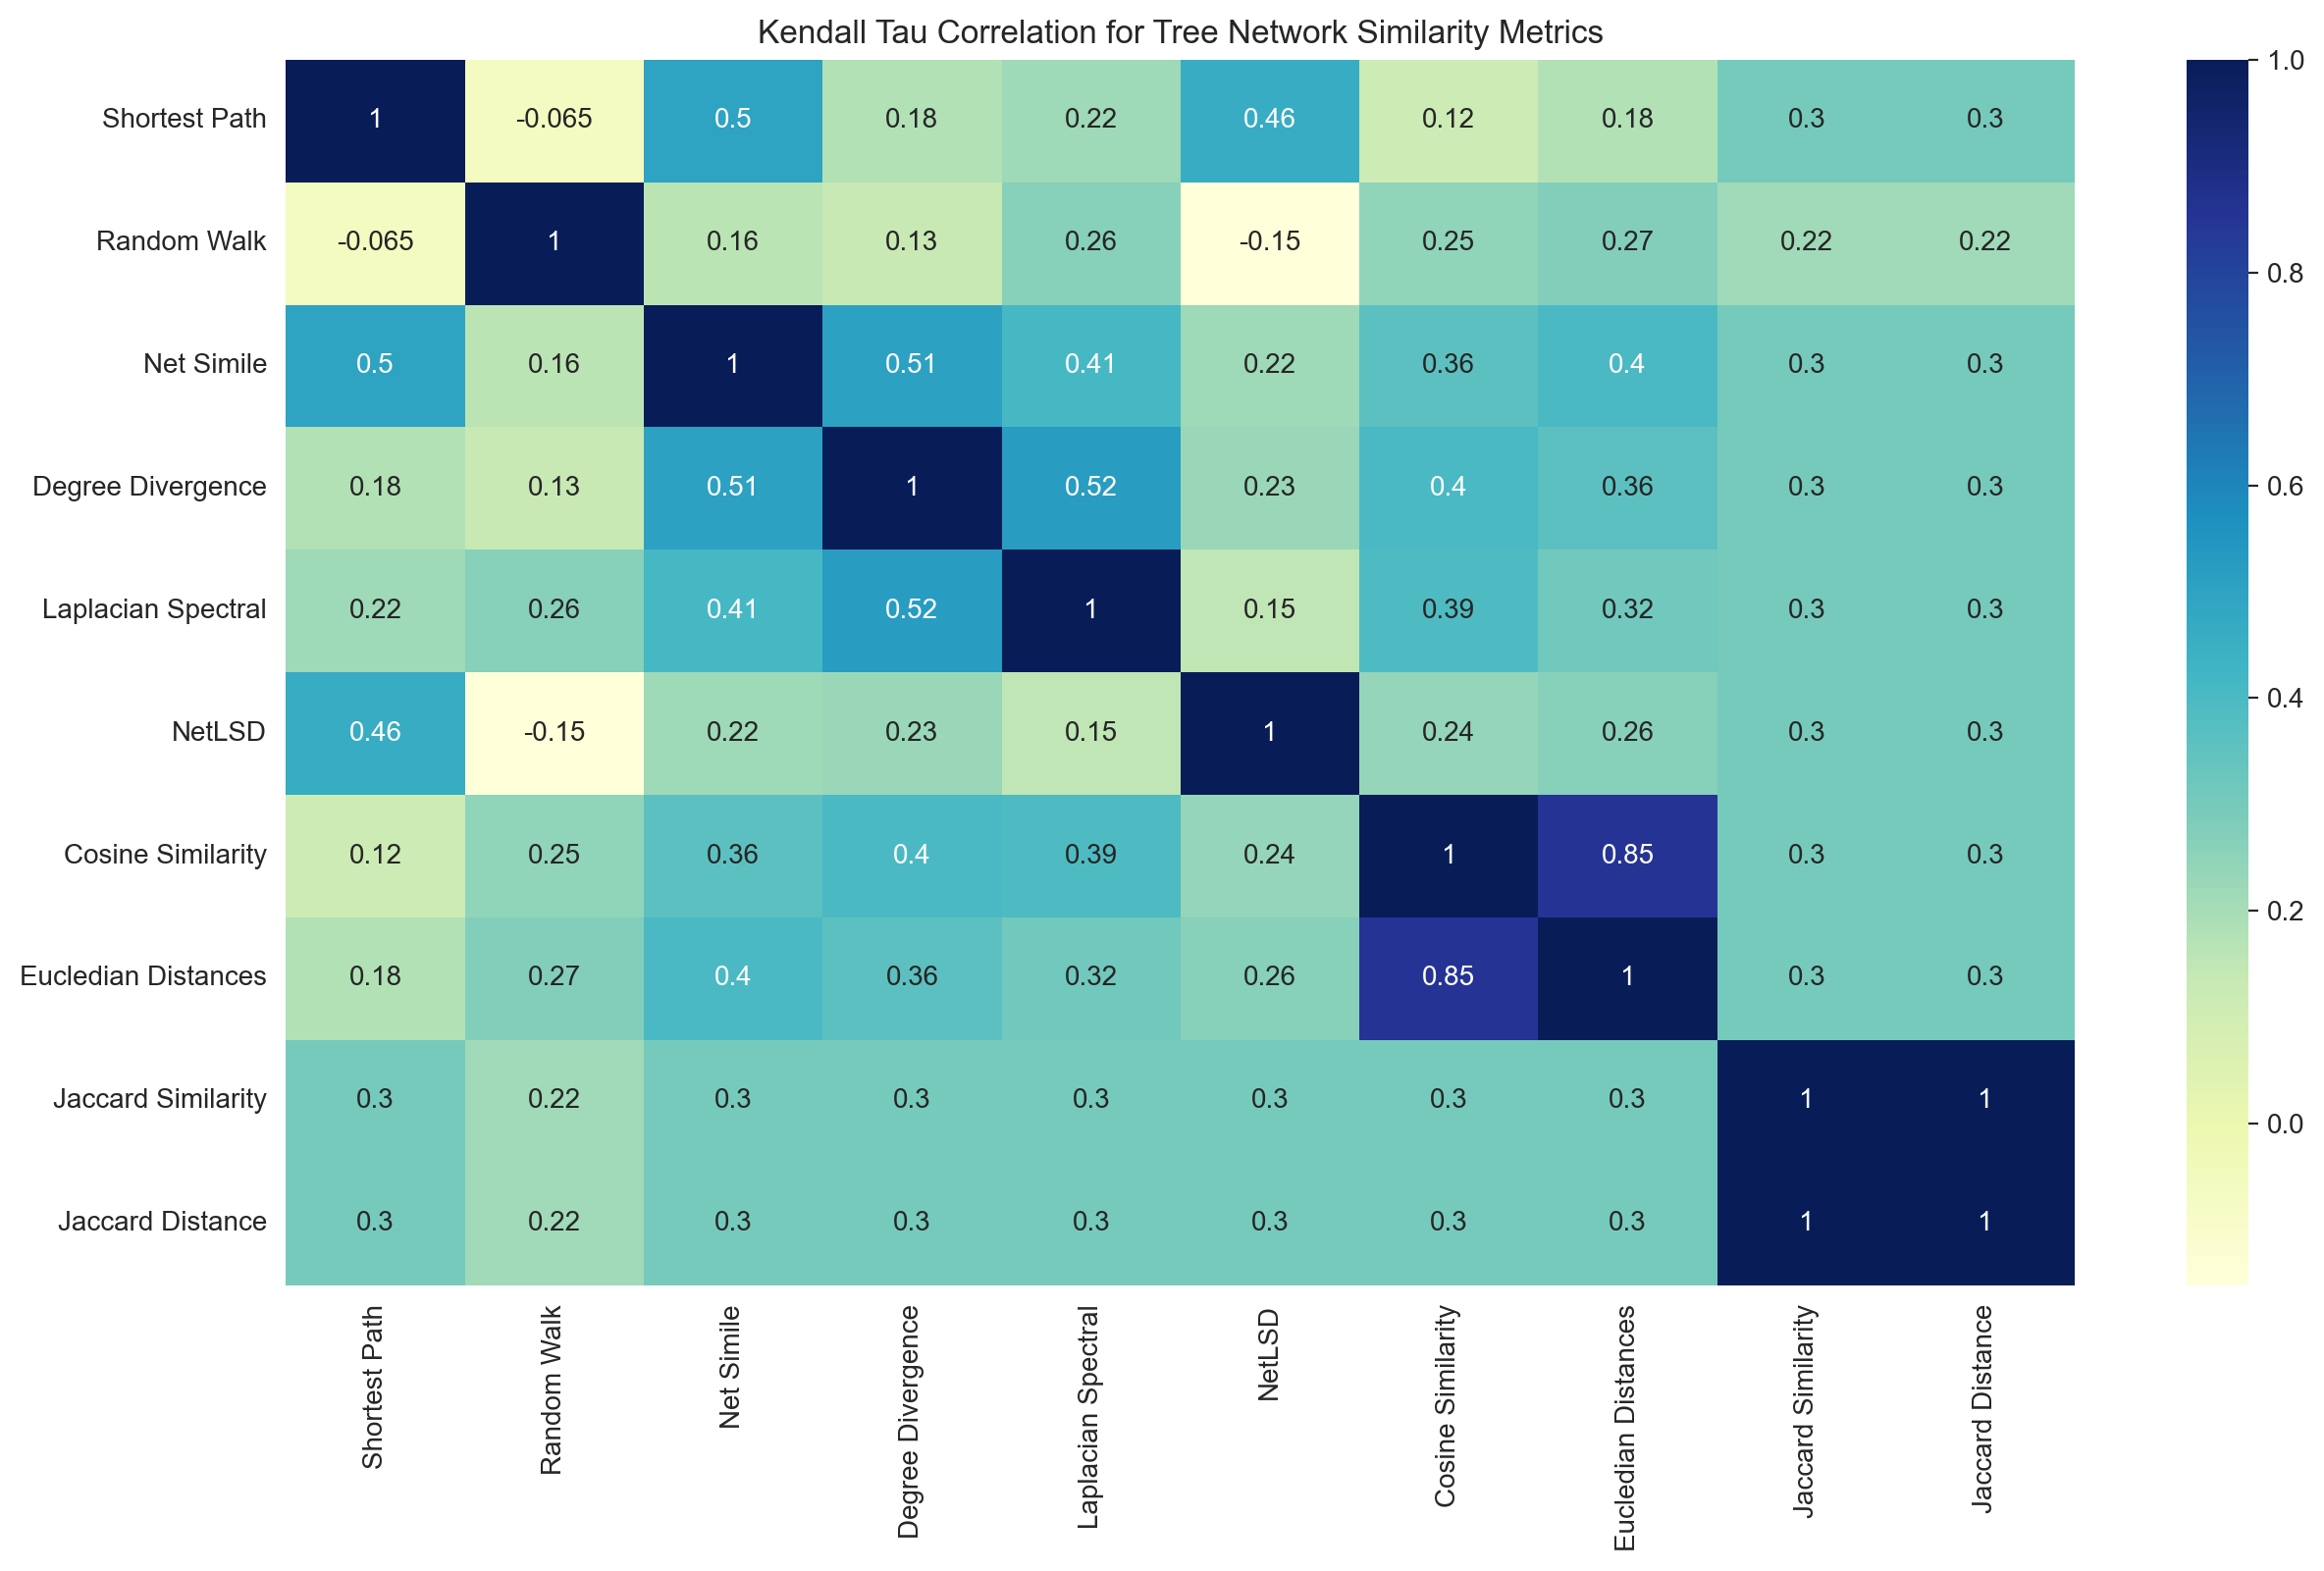
\includegraphics[width=0.85\textwidth,center]{picture/Tree/tree2.png}
\caption[Heatmap showing Kendall-Tau correlations between the road network similarity methods for Radial Road Networks]{Heatmap showing Kendall-Tau correlations between the road network similarity methods when the road network: City of Westminster, London was used as the reference network.}
\label{fig:network ranking tree}
\end{figure}

The Kendall-Tau distances between the scores generated by the different methods when comparing road networks similar to the reference network with a Tree like structure are shown in figure \ref{fig:network ranking tree}. When both the Jaccard Distance and the Jaccard Similarity are used, the results show a positive correlation of 1. This is to be expected given that the Jaccard Distance is thought to be complementary to the Jaccard Similarity, which is obtained by subtracting the Jaccard coefficient from 1. With a correlation of 0.85, the methods cosine similarity and euclidean distance also behave similarly. As shown in table \ref{tab:Road Network Similarity Methods}, both methods are vector-based and operate at the micro level. This implies that when calculating vector-based similarity on road networks at the Micro-level, either of the two methods could be used. However, there is a pronounced weaker correlation between the other methods because the level of the network they operate on and the type of comparison they use are different.

The dendrogram results are presented in the appendix section.


\section{Linear Road Network Similarity Analysis}

 The road network Sydney Australia was selected as the reference network for the Linear road similarity analysis, and the methods are used to compare the other networks to the reference network and generate a numerical similarity score. The networks are then clustered in hierarchical order. The results for this analysis are presented in Figure \ref{fig:Hierarchical Clustering Dendrogram for Linear Road Networking Similarity}.

\begin{figure}[!ht]
\centering
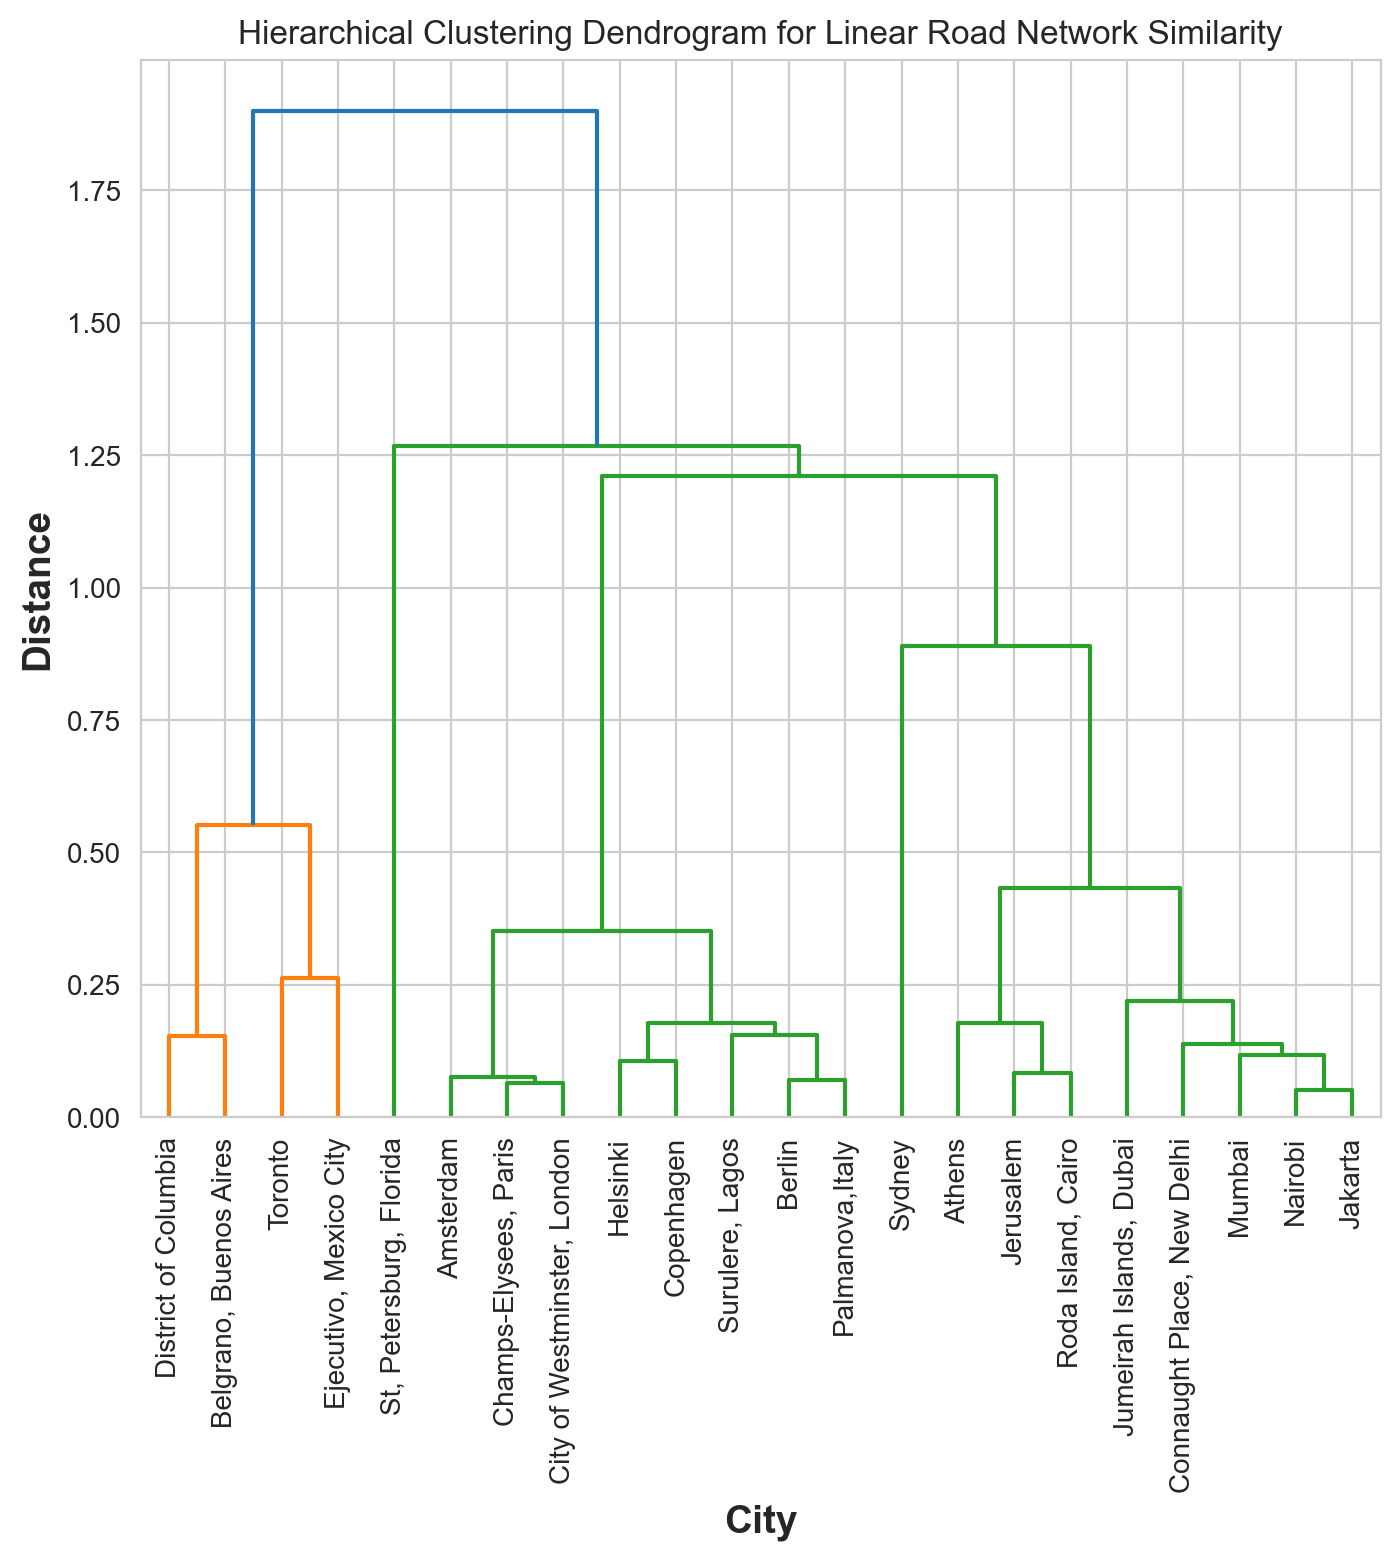
\includegraphics[width=0.75\textwidth,center]{picture/Linear/linear_dendrogram2.png}
\caption[Hierarchical Clustering Dendrogram for Linear Road Networking Similarity]{Hierarchical Clustering Dendrogram for Linear Road Networking Similarity}
\label{fig:Hierarchical Clustering Dendrogram for Linear Road Networking Similarity}
\end{figure}

Figure \ref{fig:Hierarchical Clustering Dendrogram for Linear Road Networking Similarity} presents the dendrogram obtained from the cluster analysis. The dendrogram is interpreted using the two criterias as described in Section 4.1.

For the first criteria, the dendrogram structure reveals two major clusters (Green and Orange). Using the first criterion to interpret the generated clusters, however, fails because the dendrogram results are not intuitive because some clusters contained a mix of road networks with varying structures. Except for St. Petersburg, Florida, all Road network structures identified using the Grid network analysis with the most pronounced grid-like structure are clustered together (Orange Cluster).

Interpreting the dendrogram using the second criteria, the road networks for the cities Jakarta and Nairobi are said to be clustered first based on their distances followed by the cities Champs-Elysees, Paris, City of Westminster, London  and Amsterdam, Netherlands are said to be in the same cluster based on their distance which is similar to figure \ref{fig:Hierarchical Clustering Dendrogram for Grid Road Networking Similarity}, \ref{fig:Hierarchical Clustering Dendrogram for Radial Road Networking Similarity} and \ref{fig:Hierarchical Clustering Dendrogram for Radial Road Networking Similarity} respectively which demonstrates a pattern in the similarity methods identifying the similarity between this network even when the reference networks they are compared to are changed.

In comparison to other Network Structure Analysis, the road networks: Jakarta, Jumeirah Islands, Dubai which are identified as the other only linear road network patterns in table \ref{tab:Selected Cities}, are located within the same cluster (green), but at a greater distance from the reference road network. This is to be expected because it is possible to identify the characteristics of the respective cluster and why they grouped together at a later stage by cross-checking with the similarity scores for each method included in the heatmap in figure \ref{fig:Heatmap showing the correlations for Linear Networks}.


\begin{figure}[!ht]
\centering
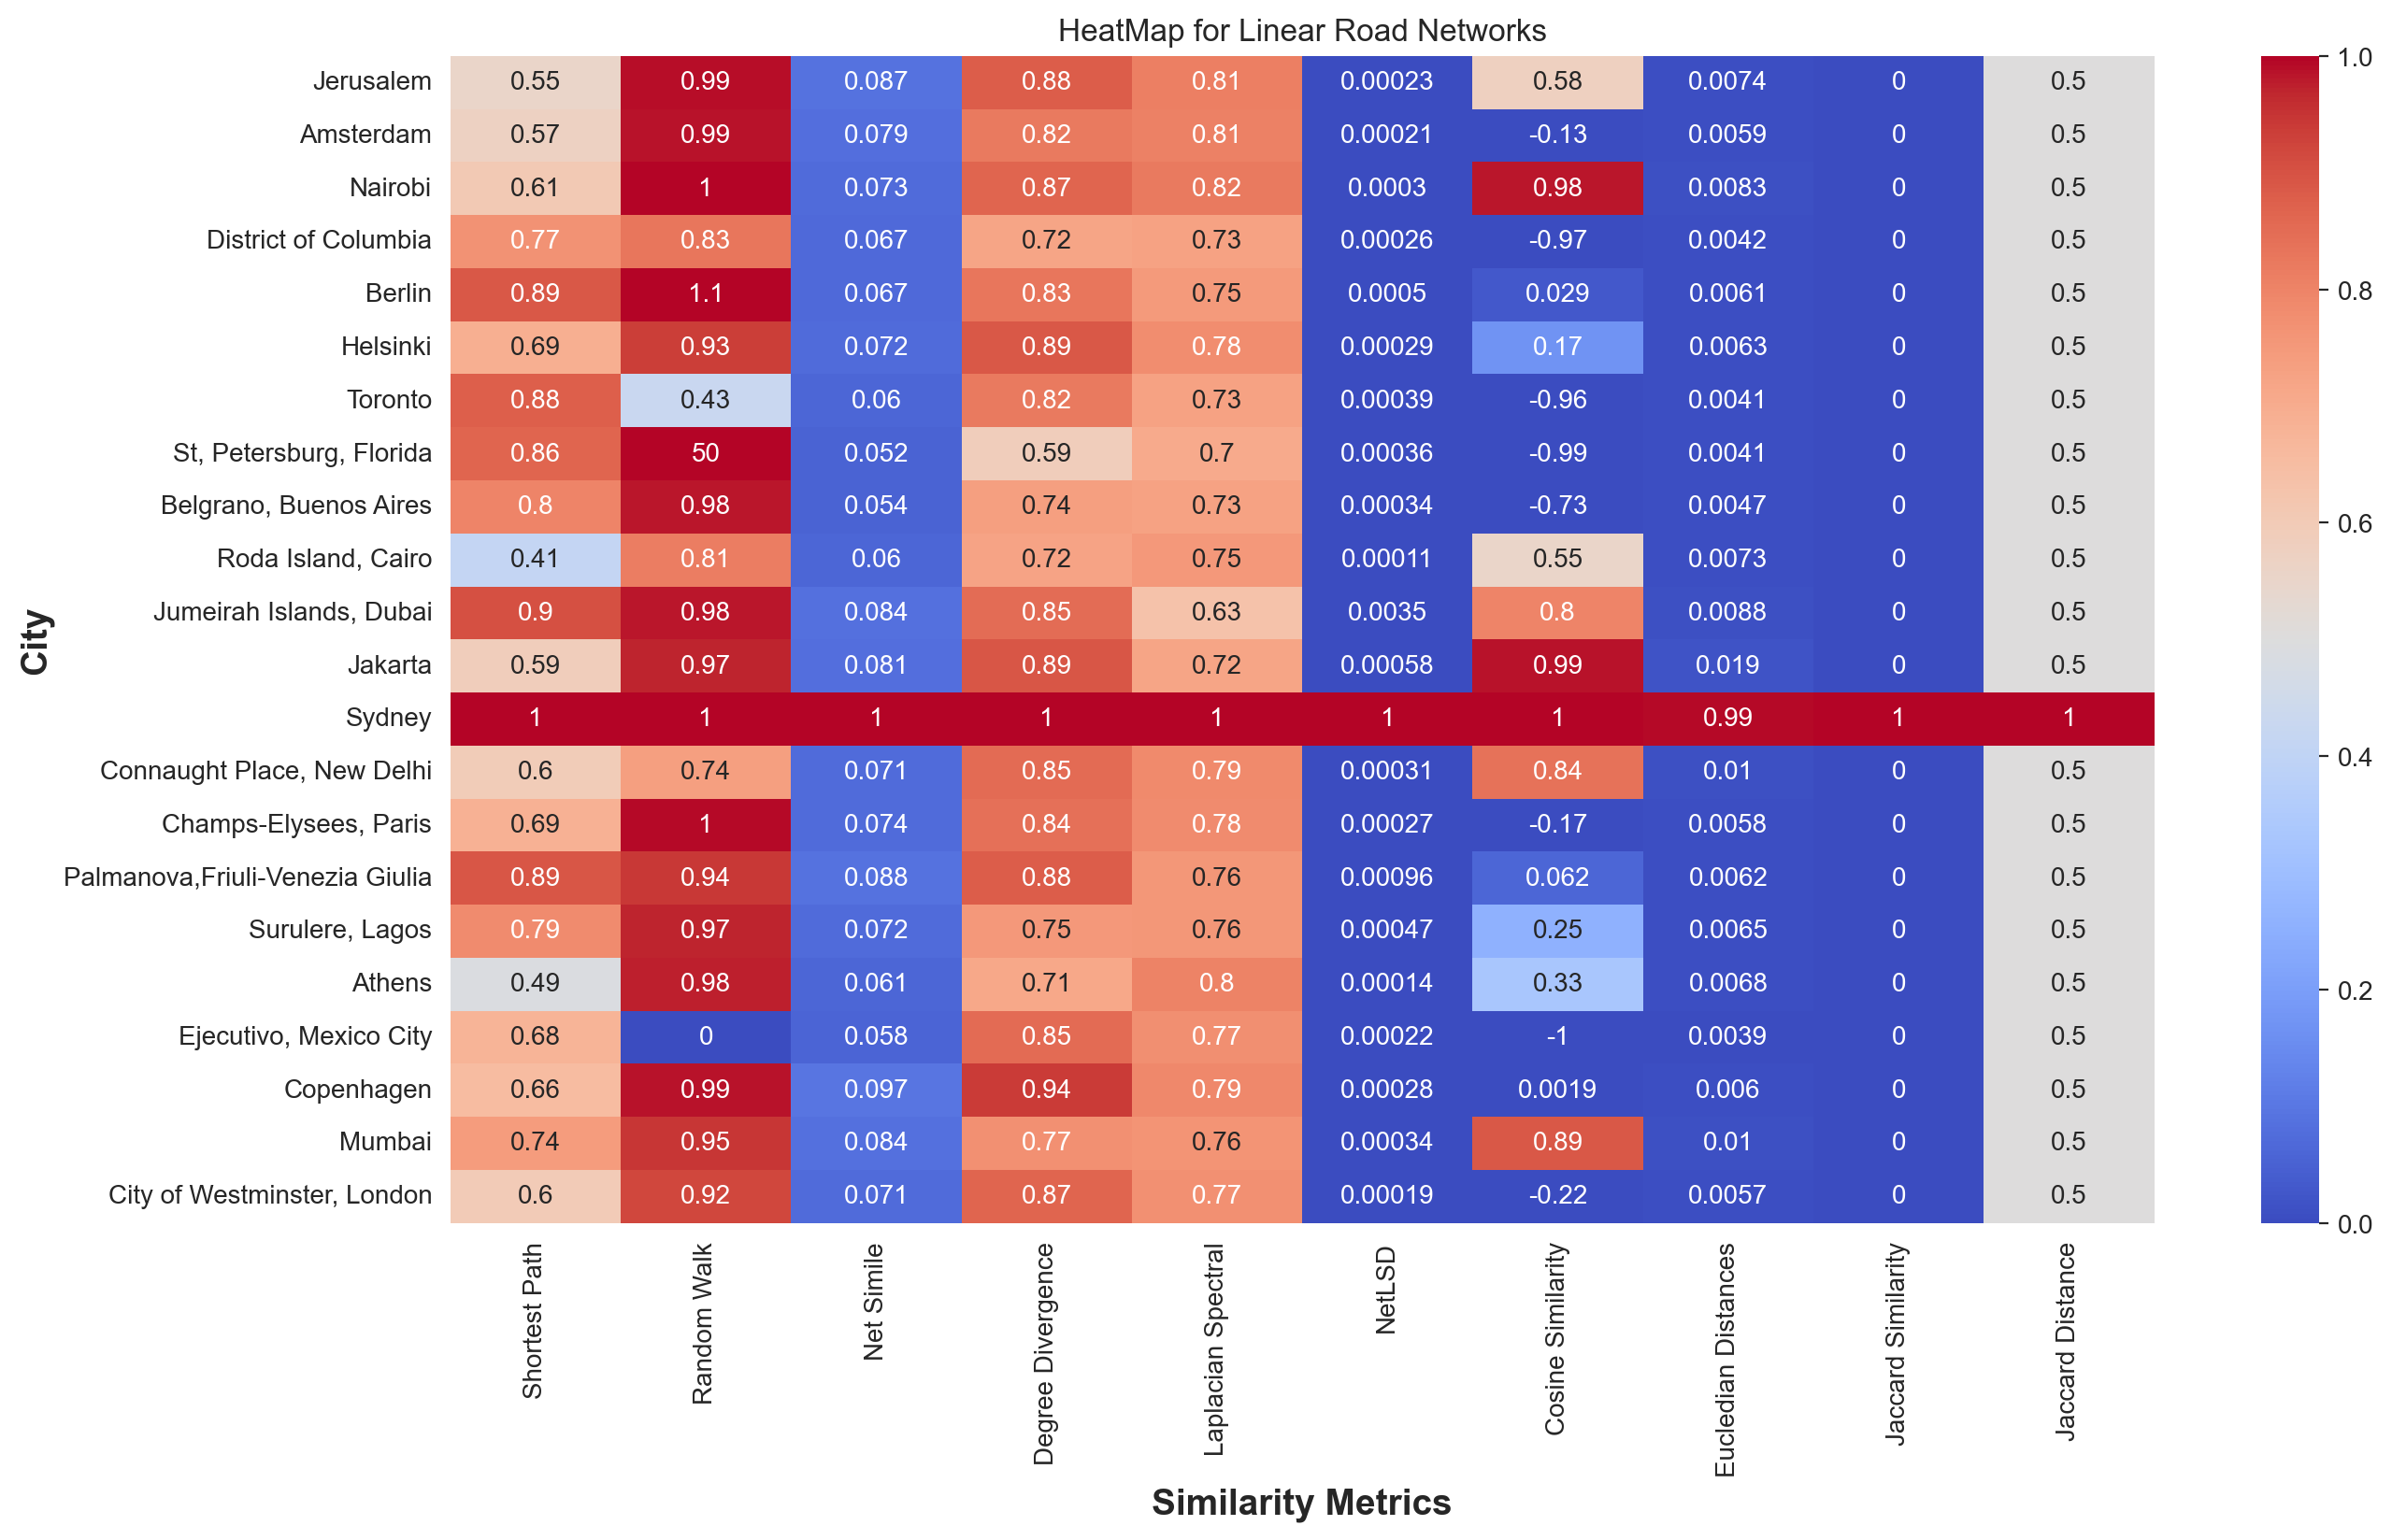
\includegraphics[width=0.85\textwidth,center]{picture/Linear/linearheatmap.png}
\caption[Heatmap showing the correlations for Linear Road Networks]{Heatmap showing the correlations between the road networks when the road network: Sydney, Australia was used as the reference network.}
\label{fig:Heatmap showing the correlations for Linear Road Networks}
\end{figure}

To find methods that behave similarly, the pairwise Kendall-Tau distance between each pair of methods is calculated first, followed by a complete-linkage hierarchical clustering because it produces a dendrogram with many small clusters, which provides insight into which groups of methods are closely correlated.

\begin{figure}[!ht]
\centering
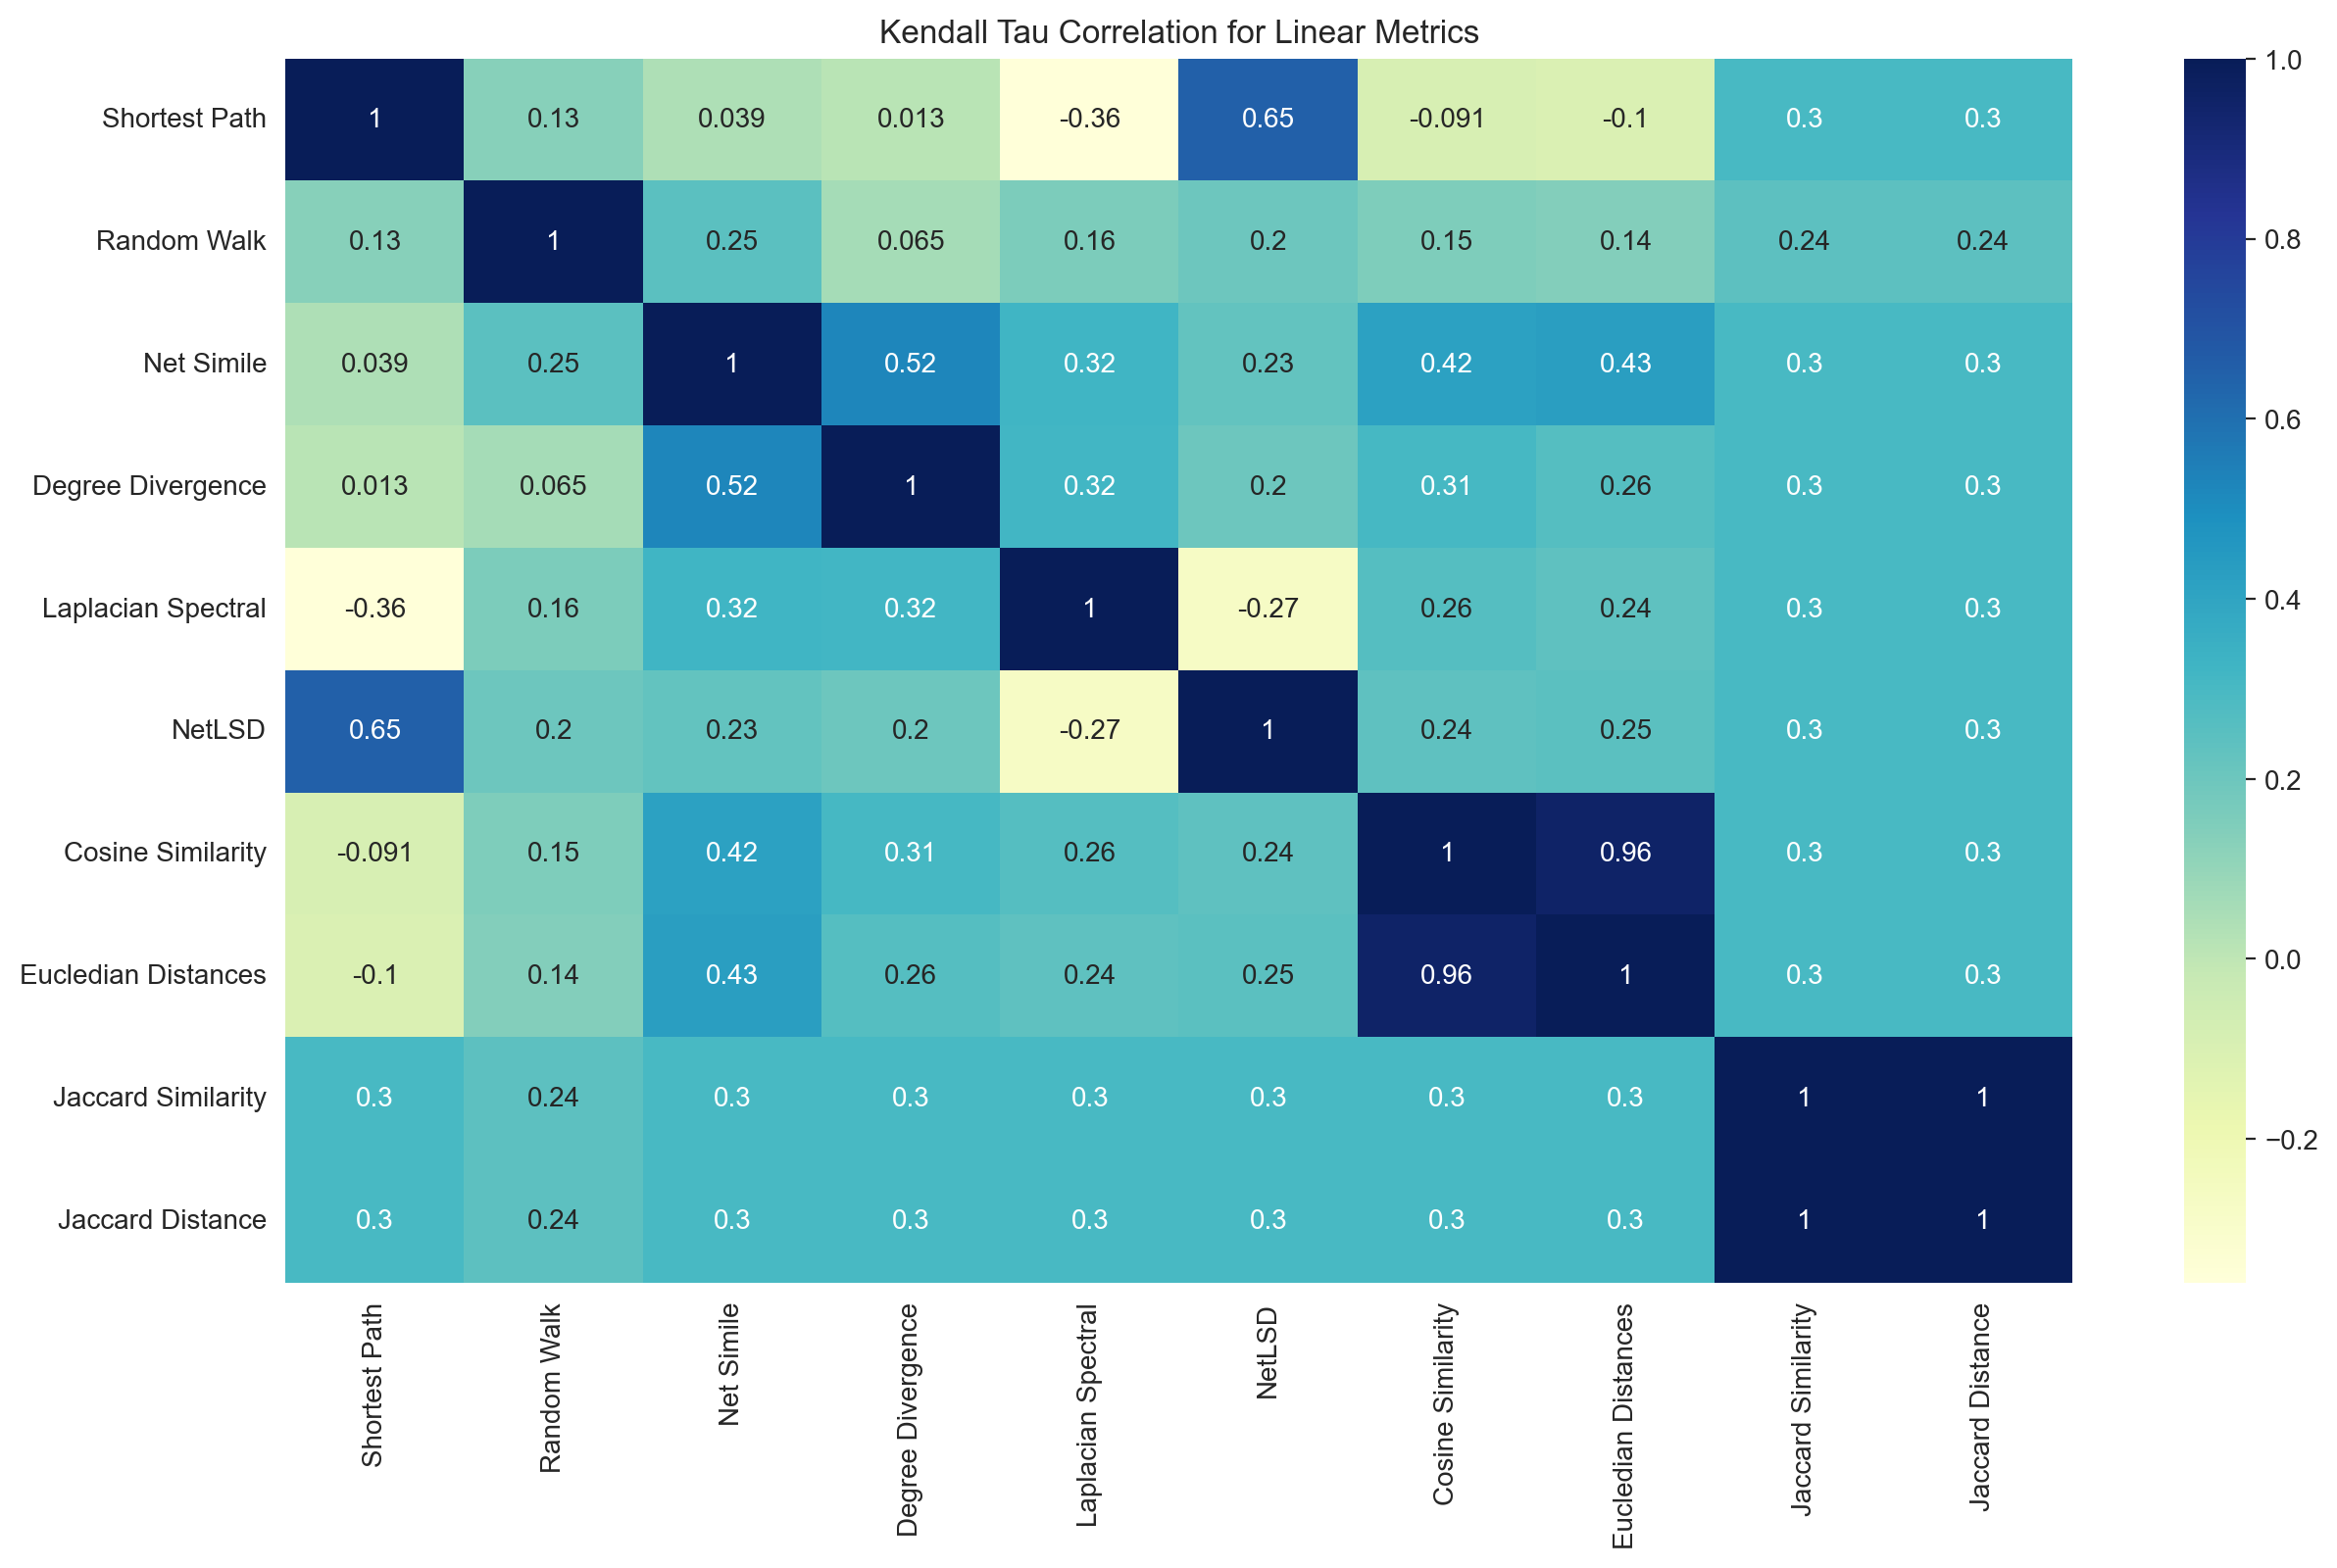
\includegraphics[width=0.85\textwidth,center]{picture/Linear/linear2.png}
\caption[Heatmap showing Kendall-Tau correlations between the road network similarity methods for Linear Road Networks]{Heatmap showing Kendall-Tau correlations between the road network similarity methods when the road network: Sydney, Australia was used as the reference network.}
\label{fig:network ranking linear}
\end{figure}

The result for the Kendall Tau distances between the scores are quite similar to the results from previous analysis only with slightly different numbers. 

The Kendall-Tau distances between the scores generated by the different methods when comparing road networks similar to the reference network with a Linear like structure are shown in figure \ref{fig:network ranking linear}. When both the Jaccard Distance and the Jaccard Similarity are used, the results show a positive correlation of 1. This is to be expected given that the Jaccard Distance is thought to be complementary to the Jaccard Similarity, which is obtained by subtracting the Jaccard coefficient from 1. With a correlation of 0.96, the methods cosine similarity and euclidean distance also behave similarly. As shown in table \ref{tab:Road Network Similarity Methods}, both methods are vector-based and operate at the micro level. This implies that when calculating vector-based similarity on road networks at the Micro-level, either of the two methods could be used. However, there is a pronounced weaker correlation between the other methods because the level of the network they operate on and the type of comparison they use are different.


\section{Cul de Sac Road Network Similarity Analysis}

The road network Jerusalem was selected as the reference network for the Cul de Sac road similarity analysis, and the methods are used to compare the other networks to the reference network and generate a numerical similarity score. The networks are then clustered in hierarchical order. The results for this analysis are presented in Figure \ref{fig:Hierarchical Clustering Dendrogram for Cul De Sac Road Networking Similarity}.

\begin{figure}[!ht]
\centering
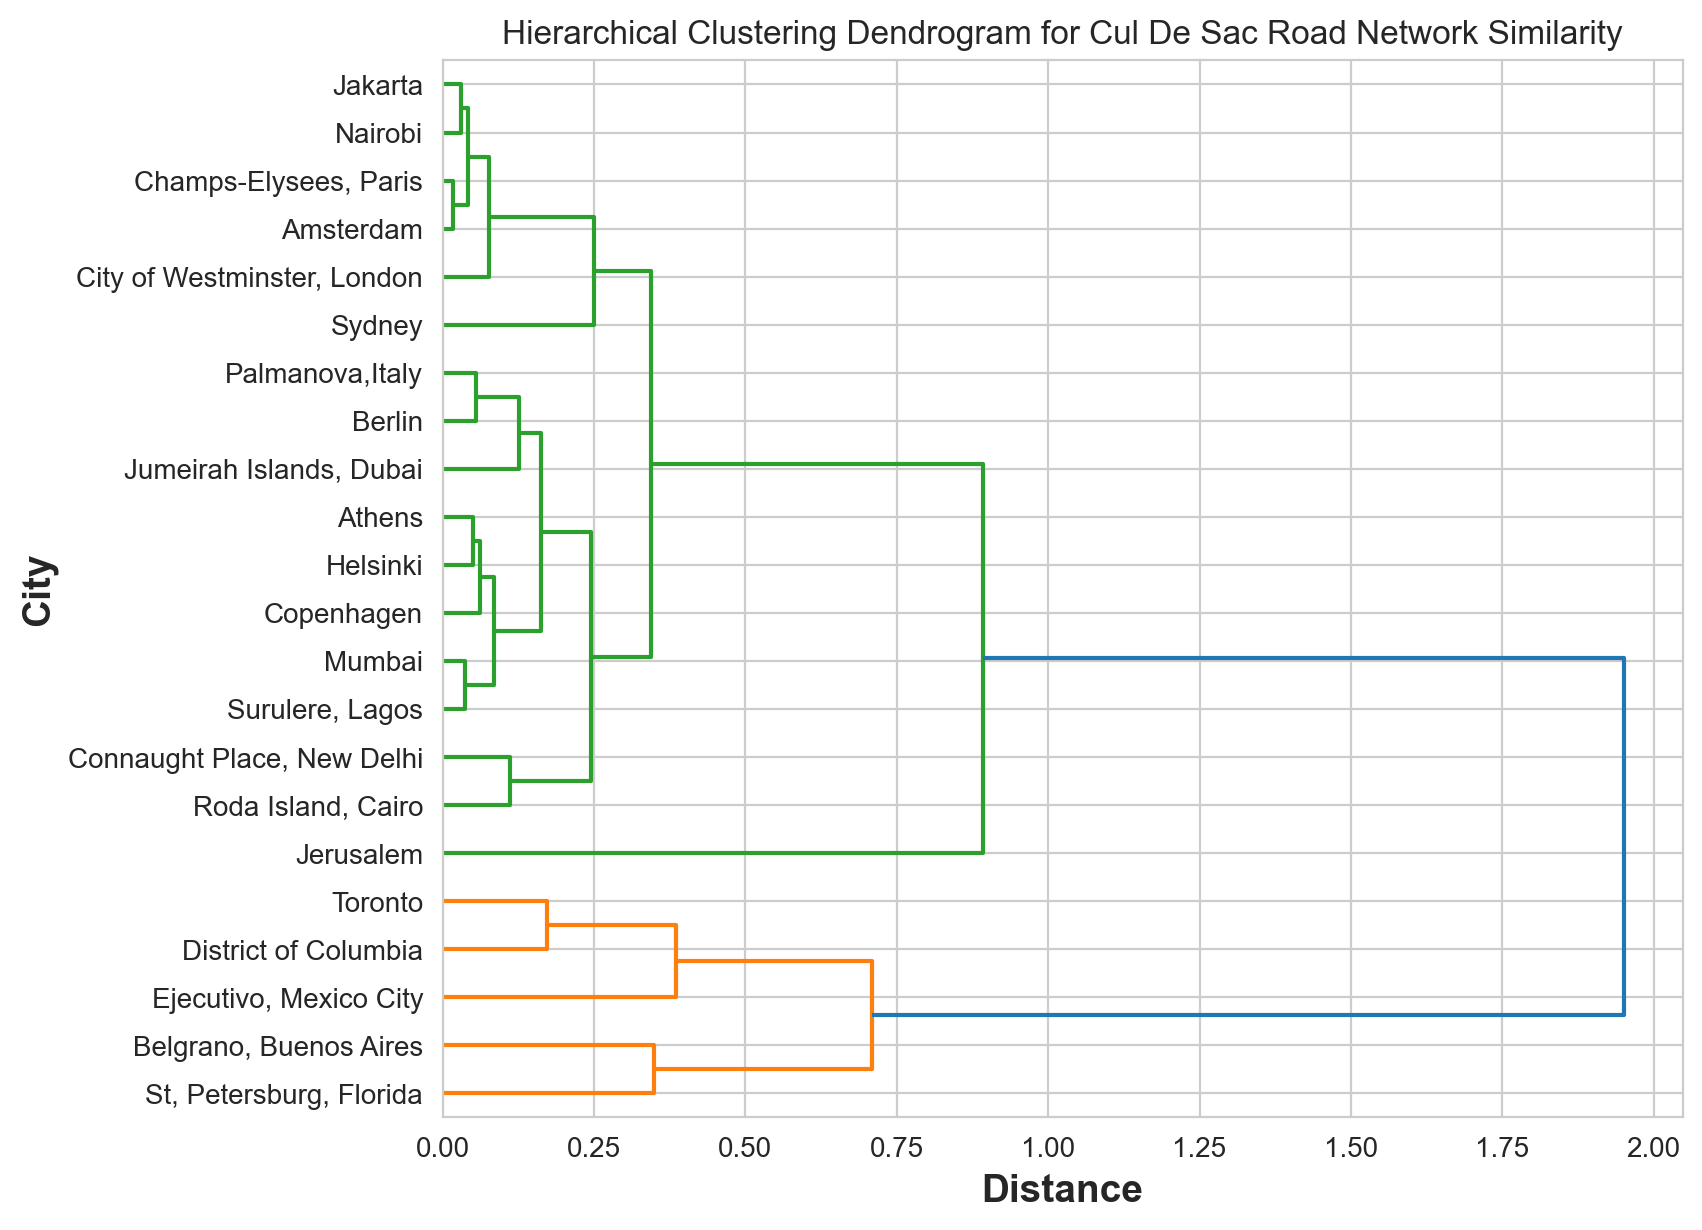
\includegraphics[width=0.75\textwidth,center]{picture/Cul De Sac/culdesac_dendrogram2.png}
\caption[Hierarchical Clustering Dendrogram for Cul De Sac Road Networking Similarity]{Hierarchical Clustering Dendrogram for Cul De Sac Road Networking Similarity}
\label{fig:Hierarchical Clustering Dendrogram for Cul De Sac Road Networking Similarity}
\end{figure}

Figure \ref{fig:Hierarchical Clustering Dendrogram for Cul De Sac Road Networking Similarity} presents the dendrogram obtained from the cluster analysis. The dendrogram is interpreted using the two criterias as described in Section 4.1.

For the first criteria, the dendrogram structure reveals two major clusters (Green and Orange). Using the first criterion to interpret the generated clusters, however, fails because the dendrogram results are not intuitive because some clusters contained a mix of road networks with varying structures. However, all Road network structures identified using the Grid network analysis with the most pronounced grid-like structure are clustered together (Orange Cluster).

Interpreting the dendrogram using the second criteria, the road networks for the cities Champs-Elysees, Paris, City of Westminster and Amsterdam, Netherland are said to be clustered first based on their distances which are similar to figures \ref{fig:Hierarchical Clustering Dendrogram for Grid Road Networking Similarity}, \ref{fig:Hierarchical Clustering Dendrogram for Radial Road Networking Similarity}, \ref{fig:Hierarchical Clustering Dendrogram for Tree Road Networking Similarity}, \ref{fig:Hierarchical Clustering Dendrogram for Linear Road Networking Similarity} and  followed by the cities Jakarta and Nairobi are said to be in the same cluster based on their distances  respectively which demonstrates a pattern in the similarity methods identifying the similarity between this networks even when the reference networks they are compared to are changed.

In comparison to other Network Analysis, the road network: Amsterdam, which is identified as the other only cul de sac road network pattern in table \ref{tab:Selected Cities}, is located within the same cluster (green), but at a greater distance from the reference road network. This is to be expected because it is possible to identify the characteristics of the respective cluster and why they are not grouped together by cross-checking with the similarity scores for each method included in the heatmap in figure \ref{fig:Heatmap showing the correlations for Tree Road Networks}.


\begin{figure}[!ht]
\centering
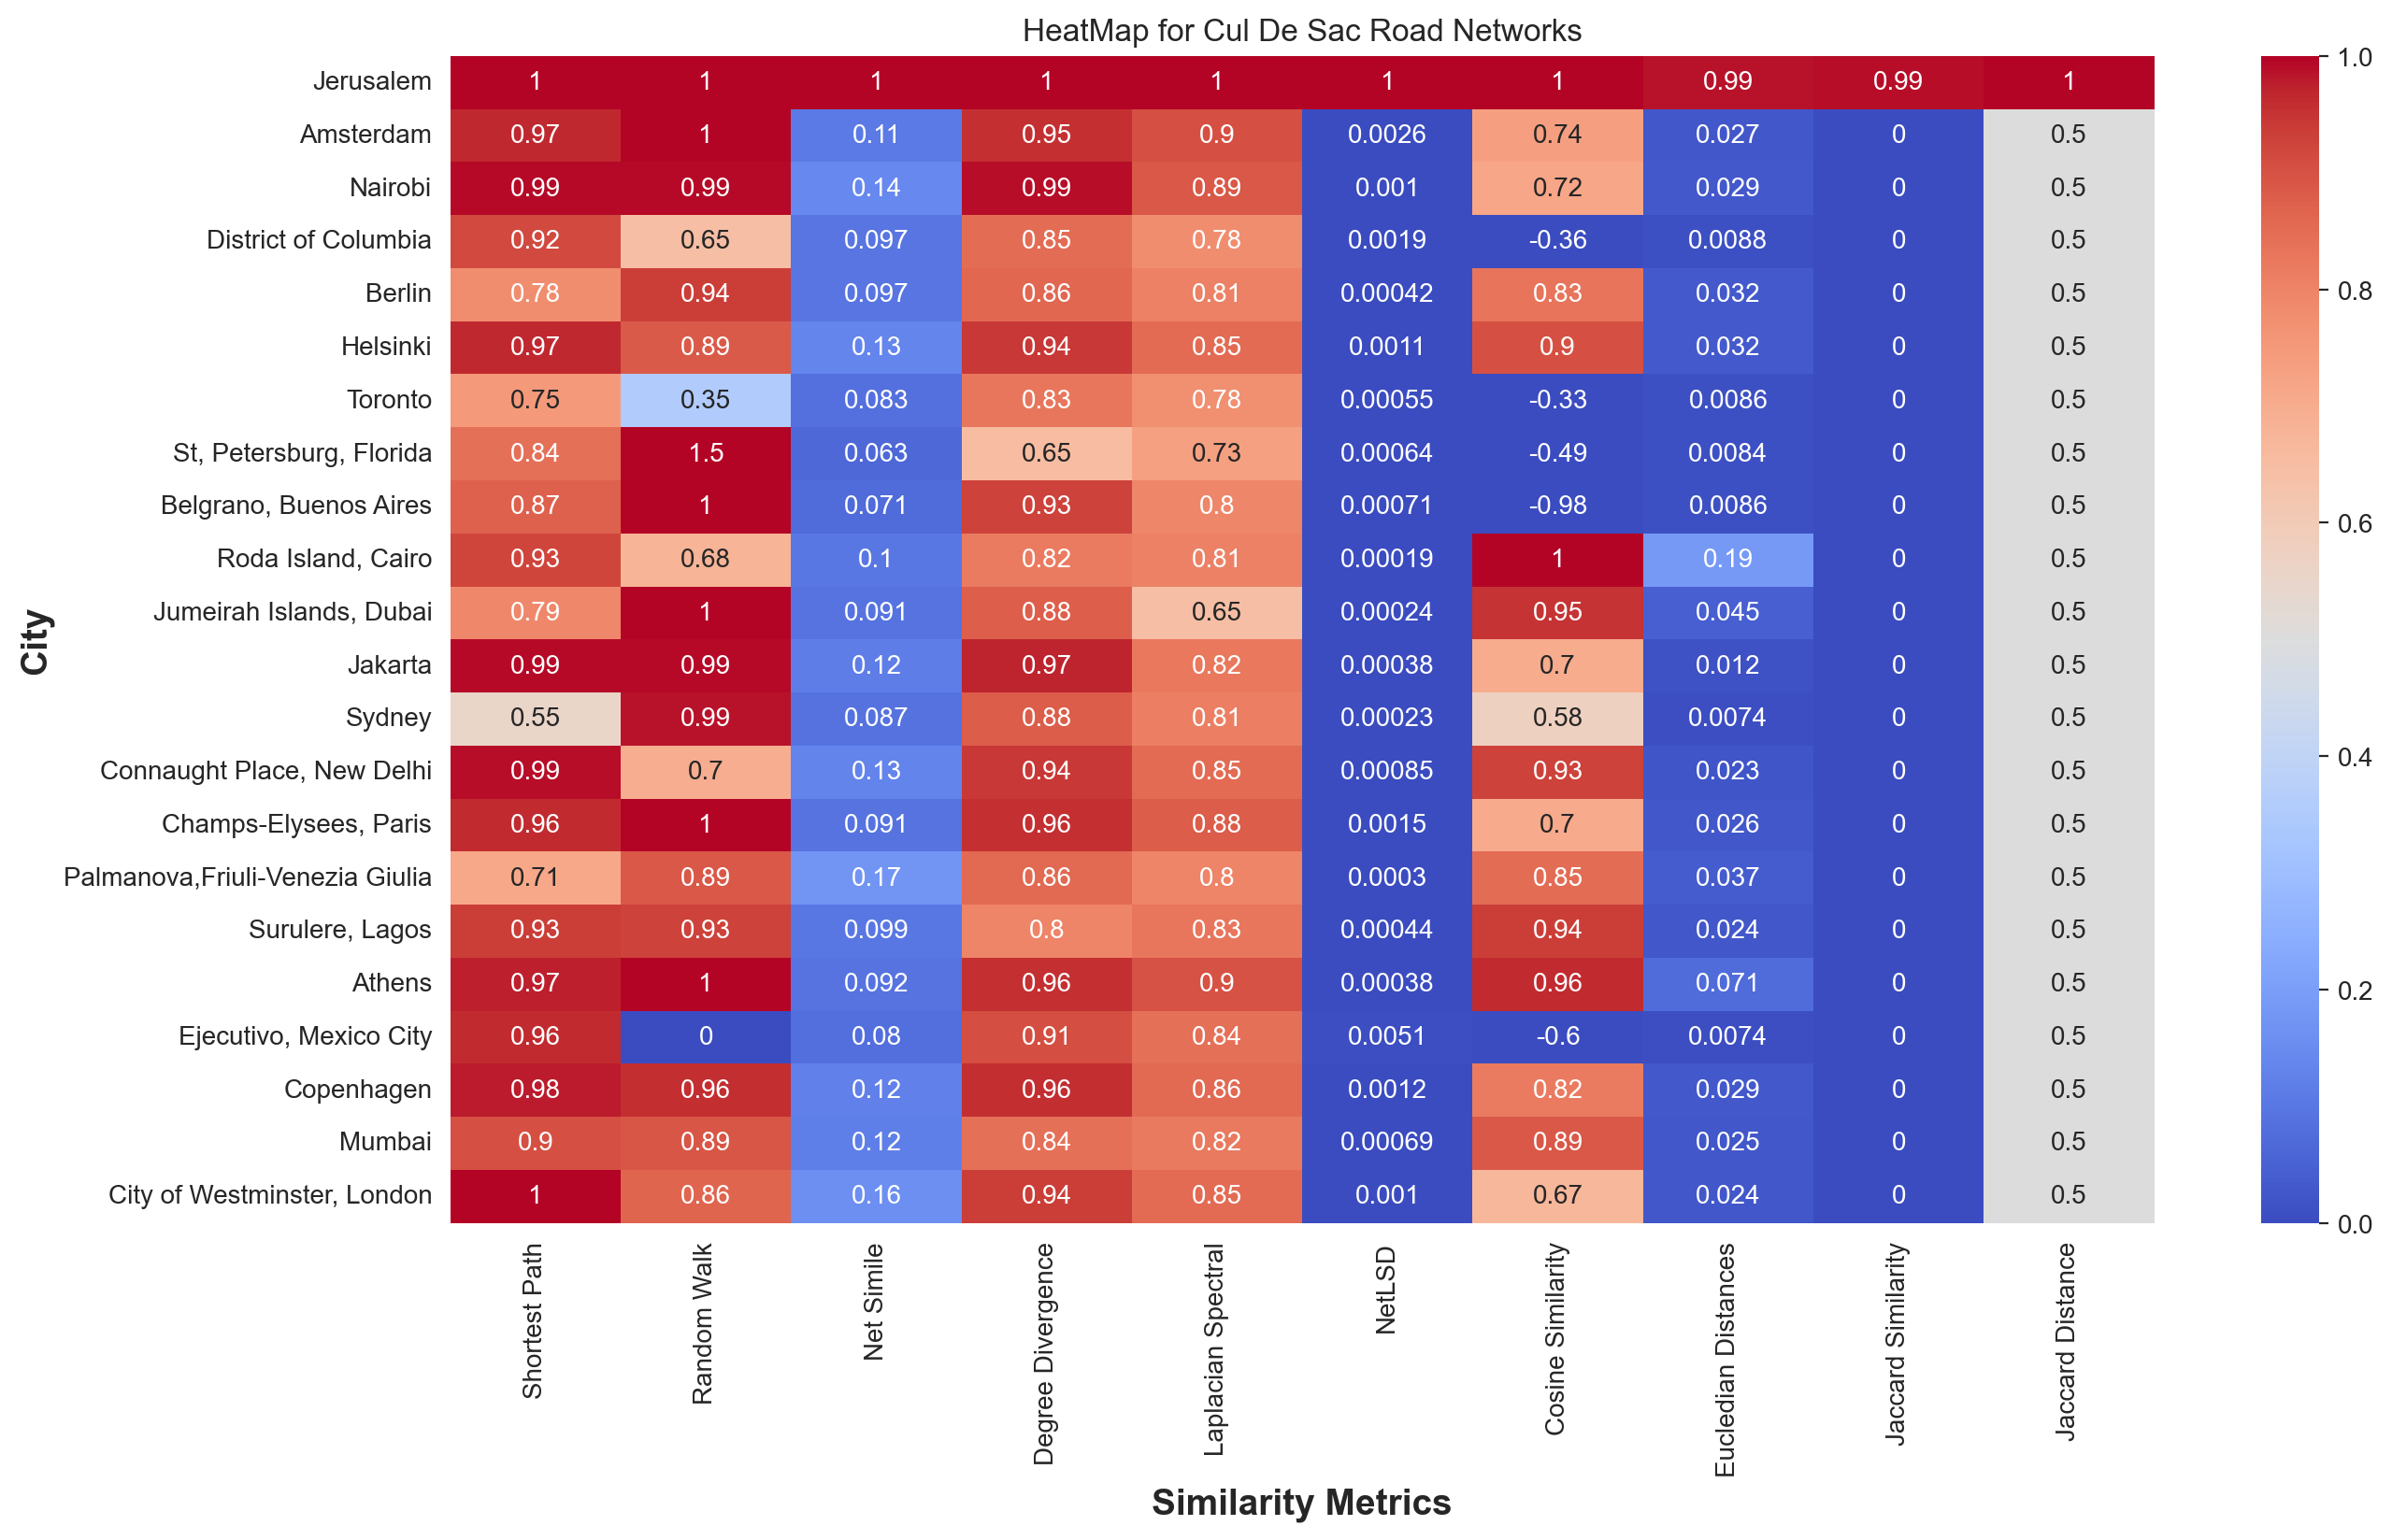
\includegraphics[width=0.85\textwidth,center]{picture/Cul De Sac/culdesacheatmap.png}
\caption[Heatmap showing the correlations for Cul De Sac Road Networks]{Heatmap showing the correlations between the road networks when the road network: Jerusalem was used as the reference network.}
\label{fig:Heatmap showing the correlations for Cul De Sac Road Networks}
\end{figure}

To find methods that behave similarly, the pairwise Kendall-Tau distance between each pair of methods is calculated first, followed by a complete-linkage hierarchical clustering because it produces a dendrogram with many small clusters, which provides insight into which groups of methods are closely correlated.

\begin{figure}[!ht]
\centering
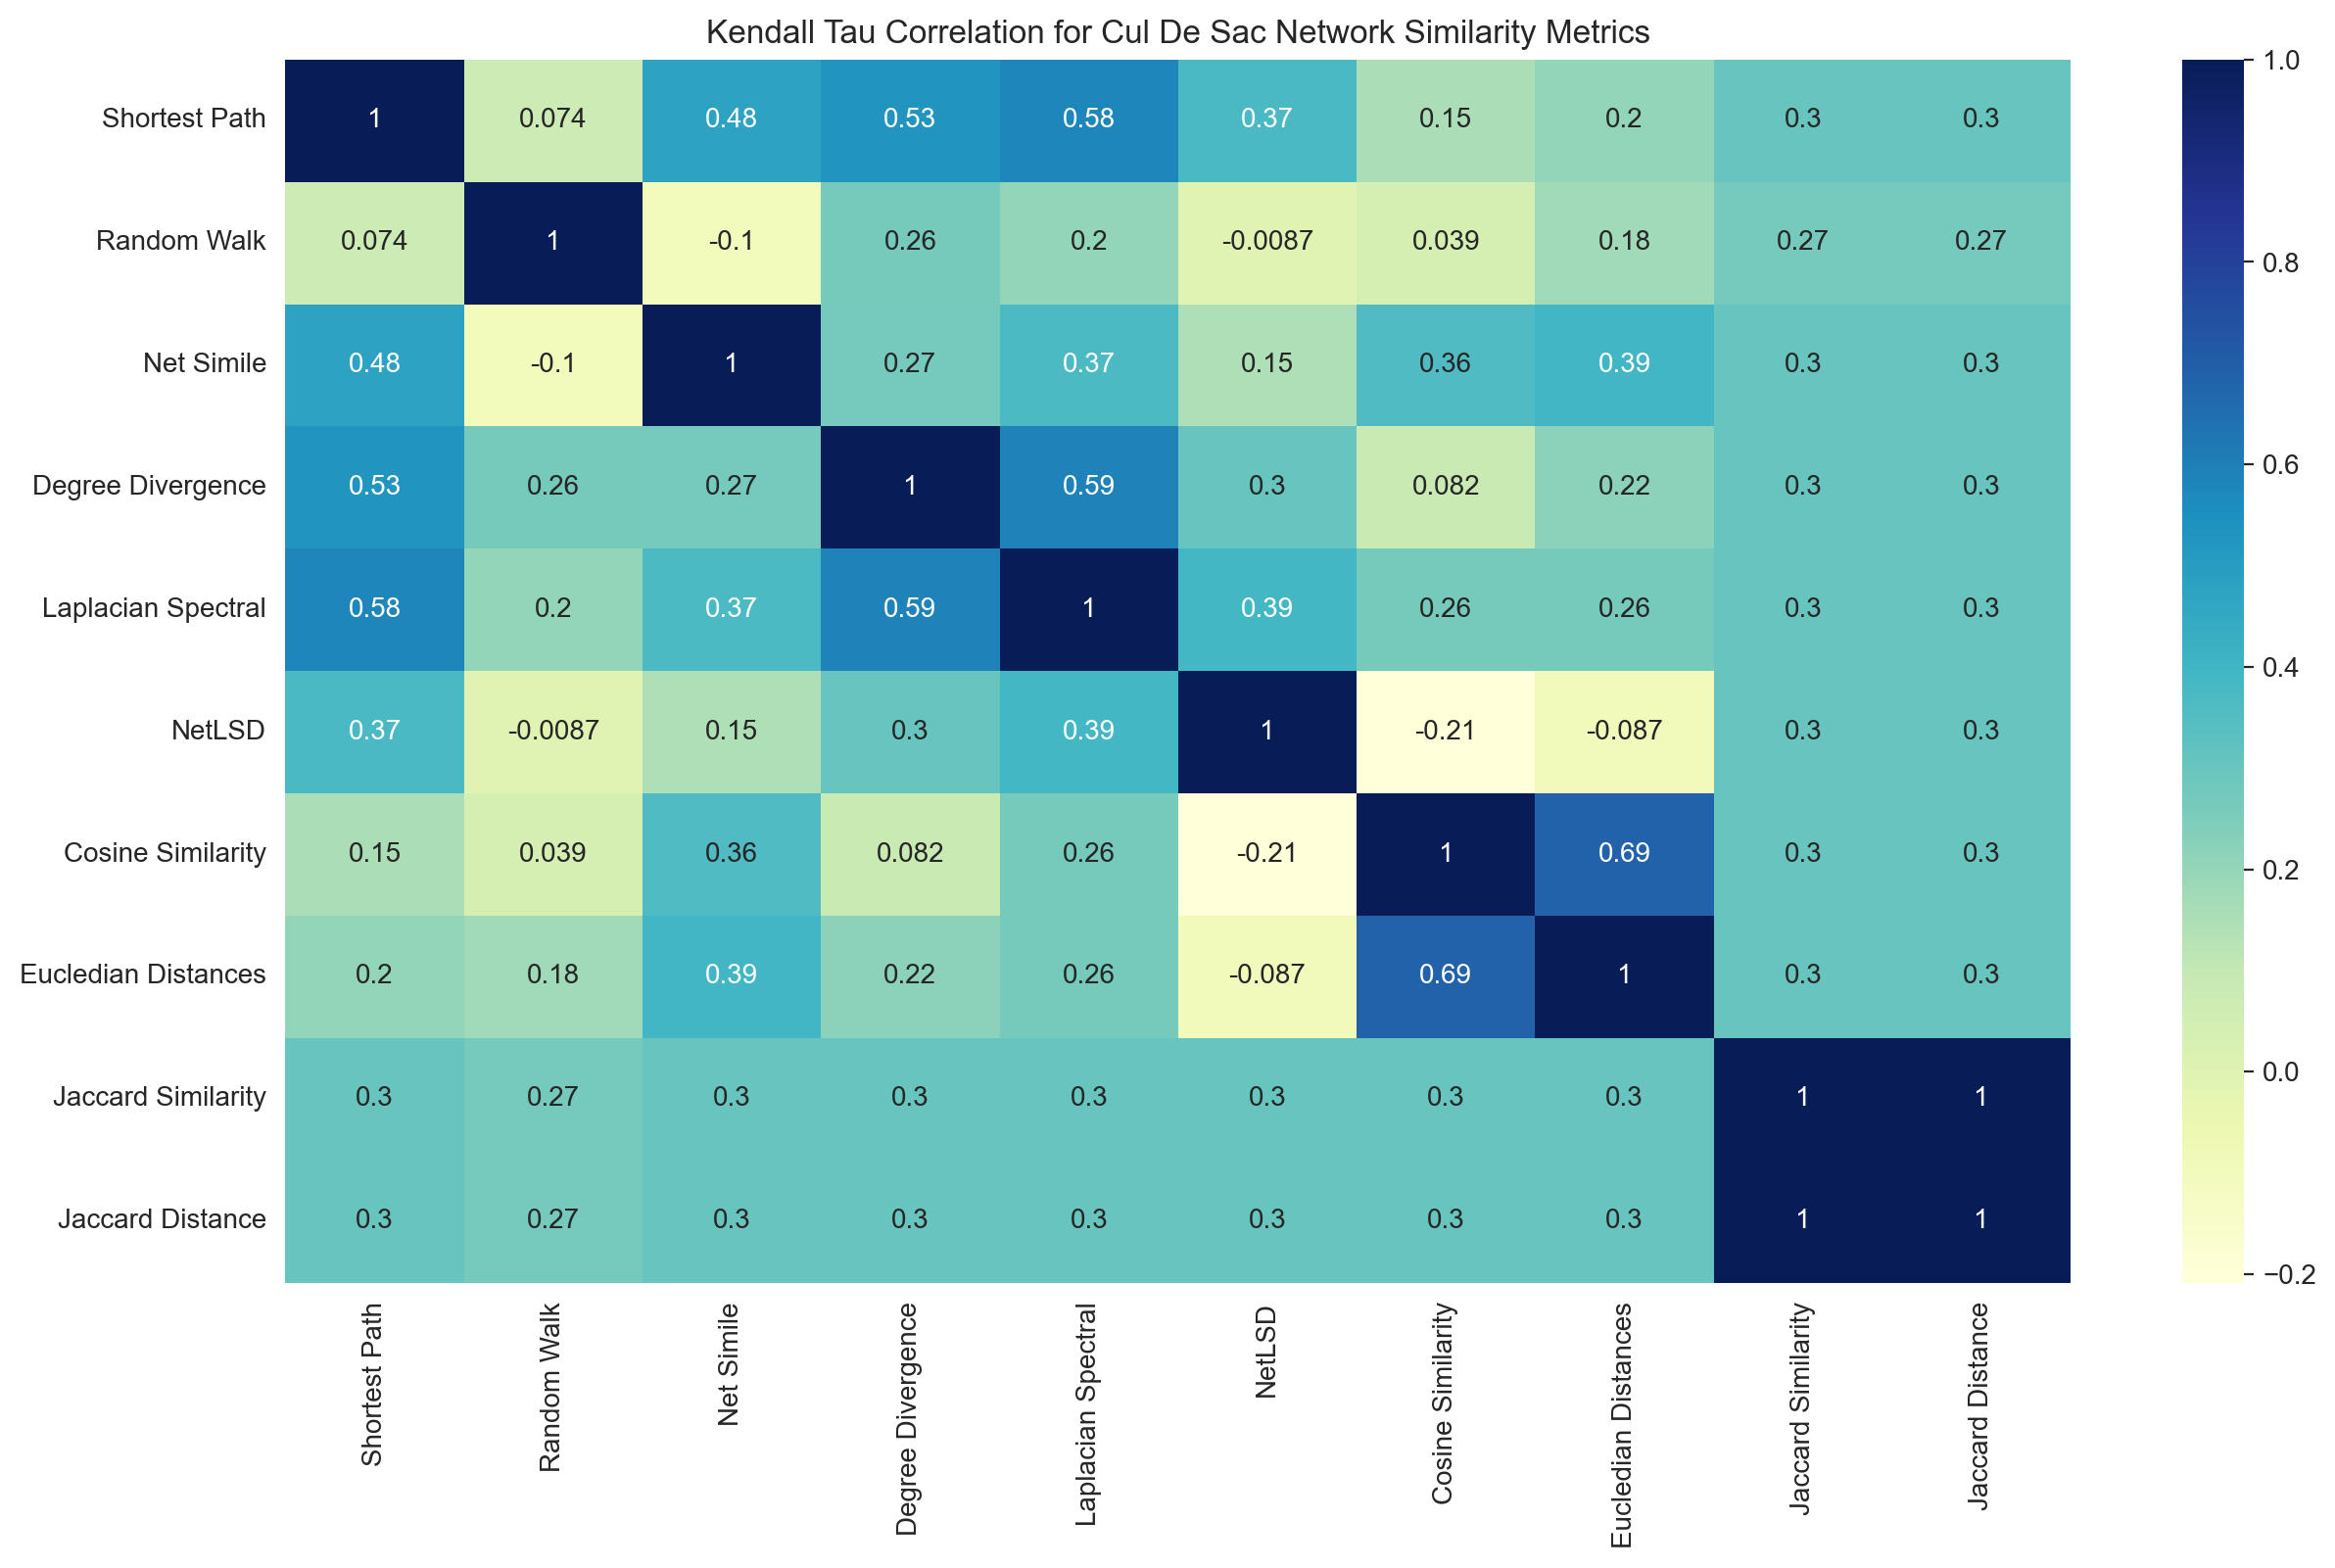
\includegraphics[width=0.85\textwidth,center]{picture/Cul De Sac/culdesac2.png}
\caption[Heatmap showing Kendall-Tau correlations between the road network similarity methods for Cul De Sac Road Networks]{Heatmap showing Kendall-Tau correlations between the road network similarity methods when the road network: Jerusalem was used as the reference network.}
\label{fig:network ranking Cul De Sac}
\end{figure}

The result for the Kendall Tau distances between the scores are quite similar to the results from previous analysis only with slightly different numbers. 

The Kendall-Tau distances between the scores generated by the different methods when comparing road networks similar to the reference network with a Tree like structure are shown in figure \ref{fig:network ranking linear}. When both the Jaccard Distance and the Jaccard Similarity are used, the results show a positive correlation of 1. This is to be expected given that the Jaccard Distance is thought to be complementary to the Jaccard Similarity, which is obtained by subtracting the Jaccard coefficient from 1. With a correlation of 0.69, the methods cosine similarity and euclidean distance behave different in comparison to other results. the reason for this change couldn't be inferred in this study but could be considered for future studies. However, there is a pronounced weaker correlation between the other methods because the level of the network they all operate on and the type of comparison they use are different.